%%%%%%%%%%%%%%%%%%%%%%%%%%%%%%%%%%%%%%%%%%%%%%%%%%%%%%%%%%%%%%%%%%%%%%%%%%
%% Review Volume (last updated on 20-4-2015)                            %%
%% Trim Size: 9in x 6in                                                 %%
%% Text Area: 7.35in (include runningheads) x 4.5in                     %%
%% Main Text: 10 on 13pt                                                %%
%% For support: Yolande Koh, <ykoh@wspc.com.sg>                         %%
%%              D. Rajesh Babu, <rajesh@wspc.com.sg>                    %%
%%%%%%%%%%%%%%%%%%%%%%%%%%%%%%%%%%%%%%%%%%%%%%%%%%%%%%%%%%%%%%%%%%%%%%%%%%
%%
%\documentclass[wsdraft]{ws-rv9x6} % to draw border line around text area
\documentclass{ws-rv9x6}
%\usepackage{subfigure}   % required only when side-by-side / subfigures are used
\usepackage{subcaption}
\usepackage{ws-rv-thm}   % comment this line when `amsthm / theorem / ntheorem` package is used
\usepackage{ws-rv-van}   % numbered citation & references (default)

\usepackage{xurl} % properly break long URLs in bibliography
\usepackage{hyperref}


%\usepackage{ws-index}   % to produce multiple indexes
\makeindex
%\newindex{aindx}{adx}{and}{Author Index}       % author index
%\renewindex{default}{idx}{ind}{Subject Index}  % subject index

\newcommand{\morecite}{{\color{red}{[citation]}}}
\newcommand{\TODO}[1]{\textcolor{red}{#1}} % for temporary working notes
\newenvironment{paraphrase}{\color{blue}}{\color{black}} % for text from old paper that needs to be paraphrased
\newcommand{\commentOut}[1]{} 
 
\begin{document}

\chapter[Evaluating Deleted File Recovery Tools per NIST Guidelines]{Evaluating Deleted File Recovery Tools per NIST Guidelines:\\ Results and Critique \label{ra_ch1}}

\author[A. Meyer and S. Roy]{Andrew Meyer and S. Roy\footnote{Author footnote.}}
%\index[aindx]{Author, F.} % or \aindx{Author, F.}
%\index[aindx]{Author, S.} % or \aindx{Author, S.}

\address{Computer Science Department, BGSU,\\
Bowling Green, Ohio, USA 43403, \\
apmeyer@bgsu.edu\footnote{Affiliation footnote.}}
 
\begin{abstract}
To carry out post-mortem investigation of cyber-crimes, 
professionals use various digital forensics (DF) tools. 
To aid in the standardization of DF tools, 
National Institute of Standards and Technology (NIST)’s 
Computer Forensics Tool Testing (CFTT) program 
has compiled a set of expectations for these tools’ behavior. 
DF tools meeting these expectations is critical for the 
integrity of forensic analysis. In this chapter, we focus 
on standardization of Deleted File Recovery (DFR) tools, 
which is a specific class of DF tools. We design a set of 
test images across widely-used file systems. 
We run extensive experiments on these test images as well as 
the test images provided by CFTT to evaluate the DFR tools, 
and to our surprise we find that many DFR tools that are available 
in the market do not fully meet the CFTT expectations. 
We report a comparative evaluation of these tools per CFTT 
expectations, which could help the user choose the right tool. 
We also identify the factors which may result in a failure for DFR tools, and
reflect on the applicability of the CFTT expectations. 
We hope that our current report will trigger more research 
on standardization of DFR tools from the researcher community.
\end{abstract}

%\markboth{Even Page Header}{Odd Page Header} % Customized running heads

\body

%\tableofcontents

\section{Introduction}\label{intro}

Nowadays government organizations as well as private enterprises encounter cyber-attacks quite frequently.
After such an attack law enforcement typically conducts a digital forensics (DF) investigation~\cite{df:news,cyber2011} 
with the goal of identifying what caused the attack, how it was executed, and who the potential perpetrators are. 
In addition to cyber-attacks, we encounter many other digital crimes, such as theft of intellectual properties, 
compromise of private data, and more. To conduct post-mortem analysis of cyber-attacks and digital crimes, forensics professionals
employ multiple DF tools. 

The success of the investigation depends on the accuracy and overall quality of DF tools.
Furthermore, as the investigation often culminates with a judicial proceeding in the court of law, integrity of DF tools 
is critical. On one hand, a court may throw out a piece of evidence if it was collected by a DF tool that does not follow the standards, 
and on the other hand, inaccurate results from a DF tool can cause improper prosecution of an innocent defendant. 
DF tools that are available in the market come from many vendors, and the government needs to keep an eye on the integrity of these tools. 
As a standardization initiative of DF tools,  Computer Forensics Tool Testing Program (CFTT)~\cite{cftt:nist} 
at National Institute of Standards and Technology (NIST) published a list of expectations for these tools. 

In this chapter, we consider standardization of Deleted File Recovery (DFR)~\cite{meta:dfr:standards,carving_standards} tools which is a special type of DF tools. 
Given a storage device, such as hard disk or a USB drive, a DF professional uses a DFR tool to search for and retrieve deleted files.
DFR tools find wide use in real-life DF investigations. For instance, after capturing a hard disk from a suspect's computer a
DF professional uses a DFR tool to retrieve the files that the suspect might have deleted to destroy some important artifacts.
A retrieved file might add critical evidence to the case in hand. In other words, success or failure of a DFR tool can sway the outcome of a case.

Depending on the working principle of DFR tools, they fall into two subtypes: \emph{Metadata-based DFR} tools and \emph{file carving} tools.
The first subtype utilizes the file system metadata (if available) to identify (a.k.a. recover) a deleted file. 
The second subtype (i.e., a file carving tool) does not rely on the file system metadata and instead utilizes the target file's 
header and footer signature for the recovery task. 
In this chapter, we consider both \emph{metadata-based DFR} tools and \emph{file carving} tools, and we evaluate them up to the NIST CFTT expectations.       

Scientific evaluation of a DFR tool is challenging because multiple factors of the given forensics scenario play a role in the tool's success or failure.
A few such factors are (a) whether the target file is fragmented, (b) whether the target file is (partially) overwritten by another file, 
(c) presence of other active or deleted files in the storage device (that hosts the files), etc.
When we compare DFR tools we make sure that these factors are the same to ensure a fair and scientific comparison.
To evaluate the file carving tools NIST CFTT portal provides a set of test images which are designed considering the above factors.
We use these test images in our study of file carving tools. 

For metadata-based DFR tools, in addition to the aforementioned factors, another factor is type of the file system (e.g. FAT vs. NTFS). 
Unfortunately, NIST CFTT does not provide any test image for evaluation of metadata-based DFR tools \cite{meta:dfr:standards}.
So, for each file system type we ourselves design a set of test images per NIST guidelines \cite{meta:dfr:standards}, considering each of the above factors independently.
In particular, we designed 14 test images for FAT and NTFS, and we claim that these cover most of the real-life scenarios.


Via extensive experiments we evaluated multiple frequently used DFR tools\footnote{We have chosen a few tools as the subject of our study, 
but such choosing does not imply authors' recommendation or endorsement of any particular tool.}, and we find that many tools do not meet one or more NIST expectations.
We find that a tool correctly retrieves the deleted file in some scenarios whereas it fails in other scenarios. Furthermore, we observe that 
two tools can perform differently on the same test image. From our experience, whenever possible, 
we strive to provide logical explanation of these behaviors. We find that in many cases 
success or failure of a tool depends on its design principle. 
For instance, a file carving tool may employ a \emph{strong match policy} to identify a deleted file, which can help prevent \emph{false positives} (when a tool retrieves garbage data instead of a real file),
but this may cause the tool to miss some deleted files. Conversely, employing a \emph{weak match policy} leads to opposite outcomes. 
 
We compare performance of the DFR tools and report a comparative analysis. In our opinion, such comparative analysis is beneficial to both DF tool 
users and vendors: it can help users choose the right DF tool, and it can help vendors identify room for improvement and their niche in the market. 
NIST CFTT publishes reports on DFR tools' performance, but only a subset of DFR tools are covered~\cite{cftt_meta_reports,cftt_carving_reports}. 
We need to expand the coverage as more and more tools come to the market.
Furthermore, some reports on the CFTT portal are on outdated version of the DFR tools, which warrants updating. 
For instance, at the time of writing, the reports on Autopsy~\cite{dhs:autopsy} and FTK~\cite{dhs:ftk}, two frequently used DF tools, came out in 2014. 
Both tools have received numerous updates since then.   

As we have tried to compare DFR tools' behavior in many test scenarios with NIST CFTT expectations, we have also gotten a first-hand experience of applicability 
of the NIST CFTT guidelines in a practical setting. For instance, we observe some situations where a tool may be held to an impossible standard.
We provide critique on applicability of the NIST CFTT~guidelines.


\commentOut{

As there are many file systems (e.g., ext4, HFS, etc.) in addition to FAT and NTFS, one might be interested to know why we chose FAT and NTFS for the current work. 
Because FAT and NTFS are very widely used on external storage devices and devices running Microsoft Windows, respectively,
real-life forensics investigation often involves these two file systems.
While we leave other file systems for future study, our current methodology could be 
extended to other file systems to make a similar study.


As a side benefit, our work leads to a few hands-on lab-modules to be used in digital forensics courses 
at BGSU, enriching the new DF specialization program in the CS department. We will also make these modules
publicly available to be used by relevant instructors at other universities.

} 

\section{Background}

We present some of the background material in this section that will prepare
us for the latter part of the chapter. 
In particular, we present an overview of metadata-based recovery and file carving. 
Then, we present the NIST CFTT expectations for such recovery tools.  


\subsection{Metadata-based Deleted File Recovery}
This recovery mechanism relies on the residual metadata of the deleted files, 
which are still present in the file system. Note that in a typical file system 
a file has some metadata in addition to the actual file content. However,
different file systems
manage the metadata in different ways.
In Section \ref{subsubsec:fat-overview} and Section \ref{subsubsec:ntfs-overview}, 
we present an overview of FAT and NTFS file systems, respectively, which is often
simplified to aid readability. 
Then, in Section \ref{subsubsec:meta-recovery}, we discuss how metadata can help in 
recovery of a deleted~file.


\subsubsection{FAT File System} \label{subsubsec:fat-overview}

For each file, the FAT file system maintains an important piece of metadata, 
which is known as a \emph{directory entry} and is of 32 bytes, containing three 
key elements: (i) name of the file (say bar.txt), (ii) size of the file, and 
(iii) index of the starting cluster that holds the file content. 
The file system maintains the index of the other clusters of the file (bar.txt) 
via a global table known as the FAT table. For each cluster in the file system, 
there is an entry in the FAT table, which holds the status 
(allocated vs. unallocated) of the cluster, and if allocated, 
it also tells us what the next cluster is. In particular, if $x^{th}$ entry is $0$, 
we infer that the cluster is unallocated. Otherwise, if $x^{th}$ entry is $y$, then 
that means the next cluster after cluster $x$ (as part of the same file) is $y$.
When $x^{th}$ entry holds a special value called EOF, we infer that cluster $x$ is
the last cluster of a file.

For instance, Figure~\ref{fig:fat1} illustrates the directory entry and data clusters of 
a file bar.txt. The FAT table is also shown. We can infer from the FAT table that the file's
(bar.txt) content is stored in contiguous clusters, from cluster 200 to cluster 204.


\begin{figure}[h]
     \centering
     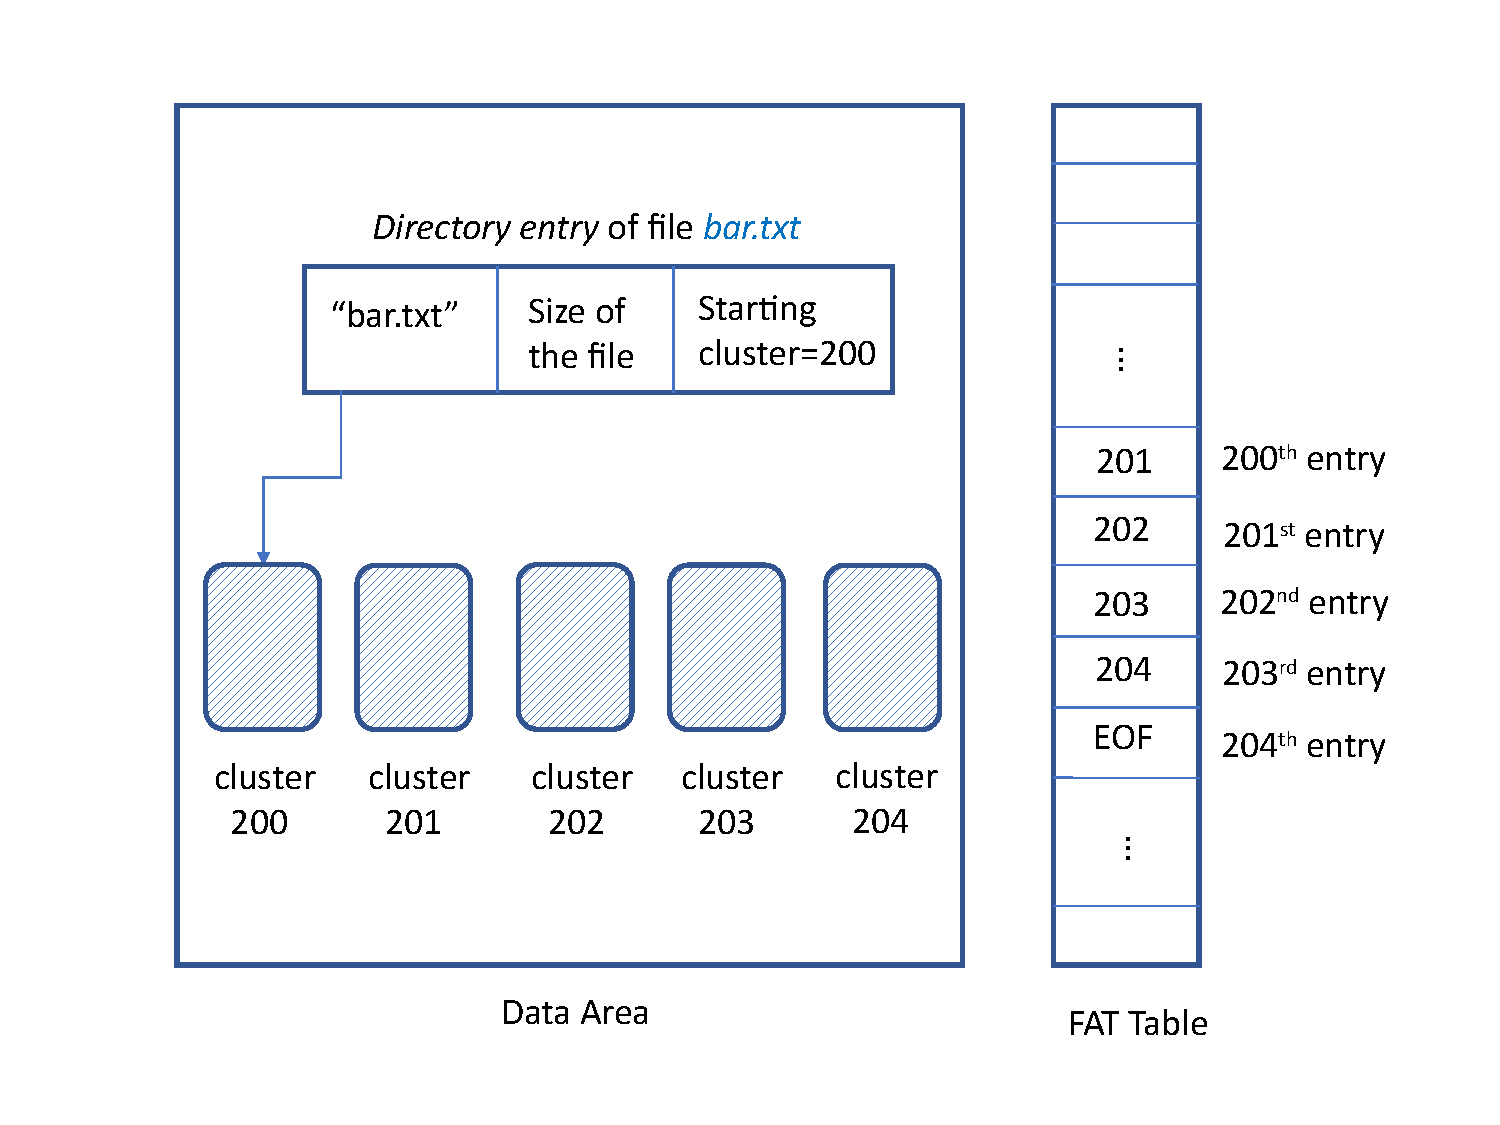
\includegraphics[width=\linewidth]{fig/fat1.pdf}
     \caption{The actual data part and metadata of file bar.txt in a FAT file system. The \emph{directory entry} of this file and the actual file content clusters (shaded) are shown on the left. The FAT table is shown on the riight.}
     \label{fig:fat1}
 \end{figure}

When a file is deleted in FAT system, most of the actual content and metadata might 
remain intact in many cases. 
Figure~\ref{fig:fat2} illustrates the status of the file system after the file bar.txt is deleted.
All fields of the directory entry remain unchanged except the first character of the file name 
is replaced with an underscore (`\_') to flag the \emph{deleted} status. The main change happens in the FAT table where all entries
that were associated with bar.txt are \emph{zeroed}. However, the clusters (holding the file content) 
remain intact until some other file (partially or fully) \emph{overwrites} them. 

  
\begin{figure}[h]
    \centering
    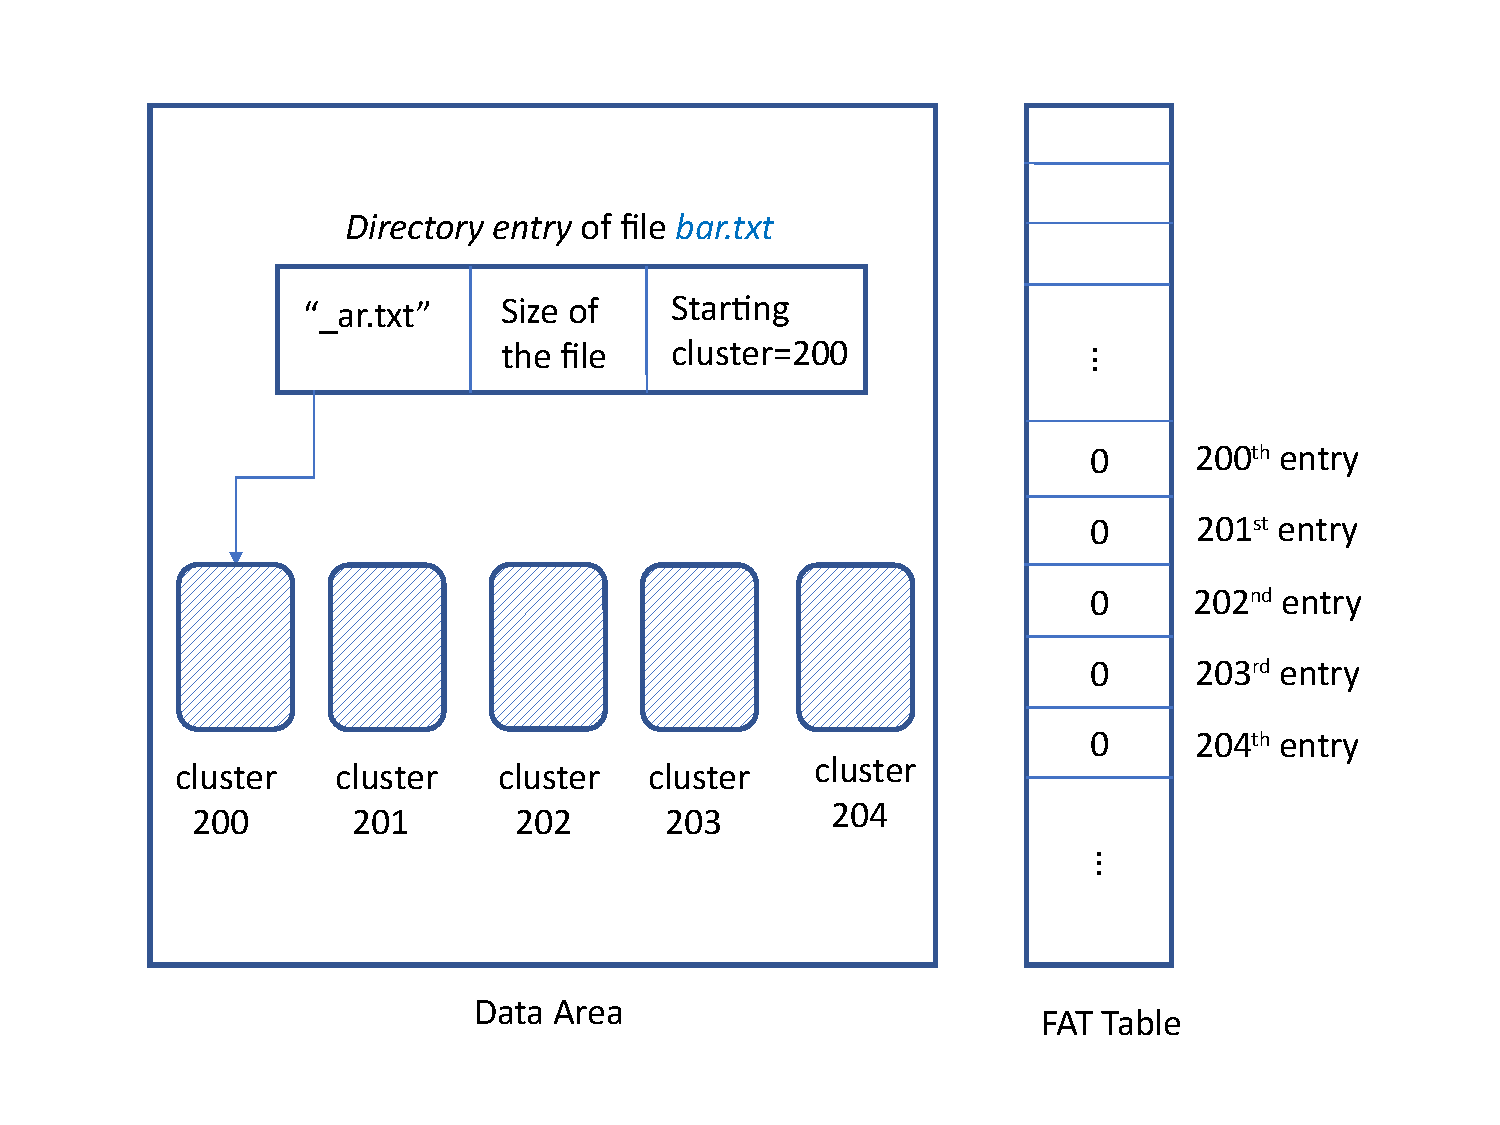
\includegraphics[width=\linewidth]{fig/fat2.pdf}
    \caption{The actual data part and metadata of bar.txt after the file is deleted whereas its entries in the FAT table (i.e., $200$th entry to $204$th entry) are~zeroed.}
    \label{fig:fat2}
\end{figure}

So far, we have considered a file whose actual content is stored in contiguous clusters. 
It is also possible that a file's content is not stored in contiguous clusters, and such a file is 
called a \emph{fragmented} file. Figure~\ref{fig:fat3} illustrates an example where file bar.txt is fragmented.

 \begin{figure}[h]
     \centering
     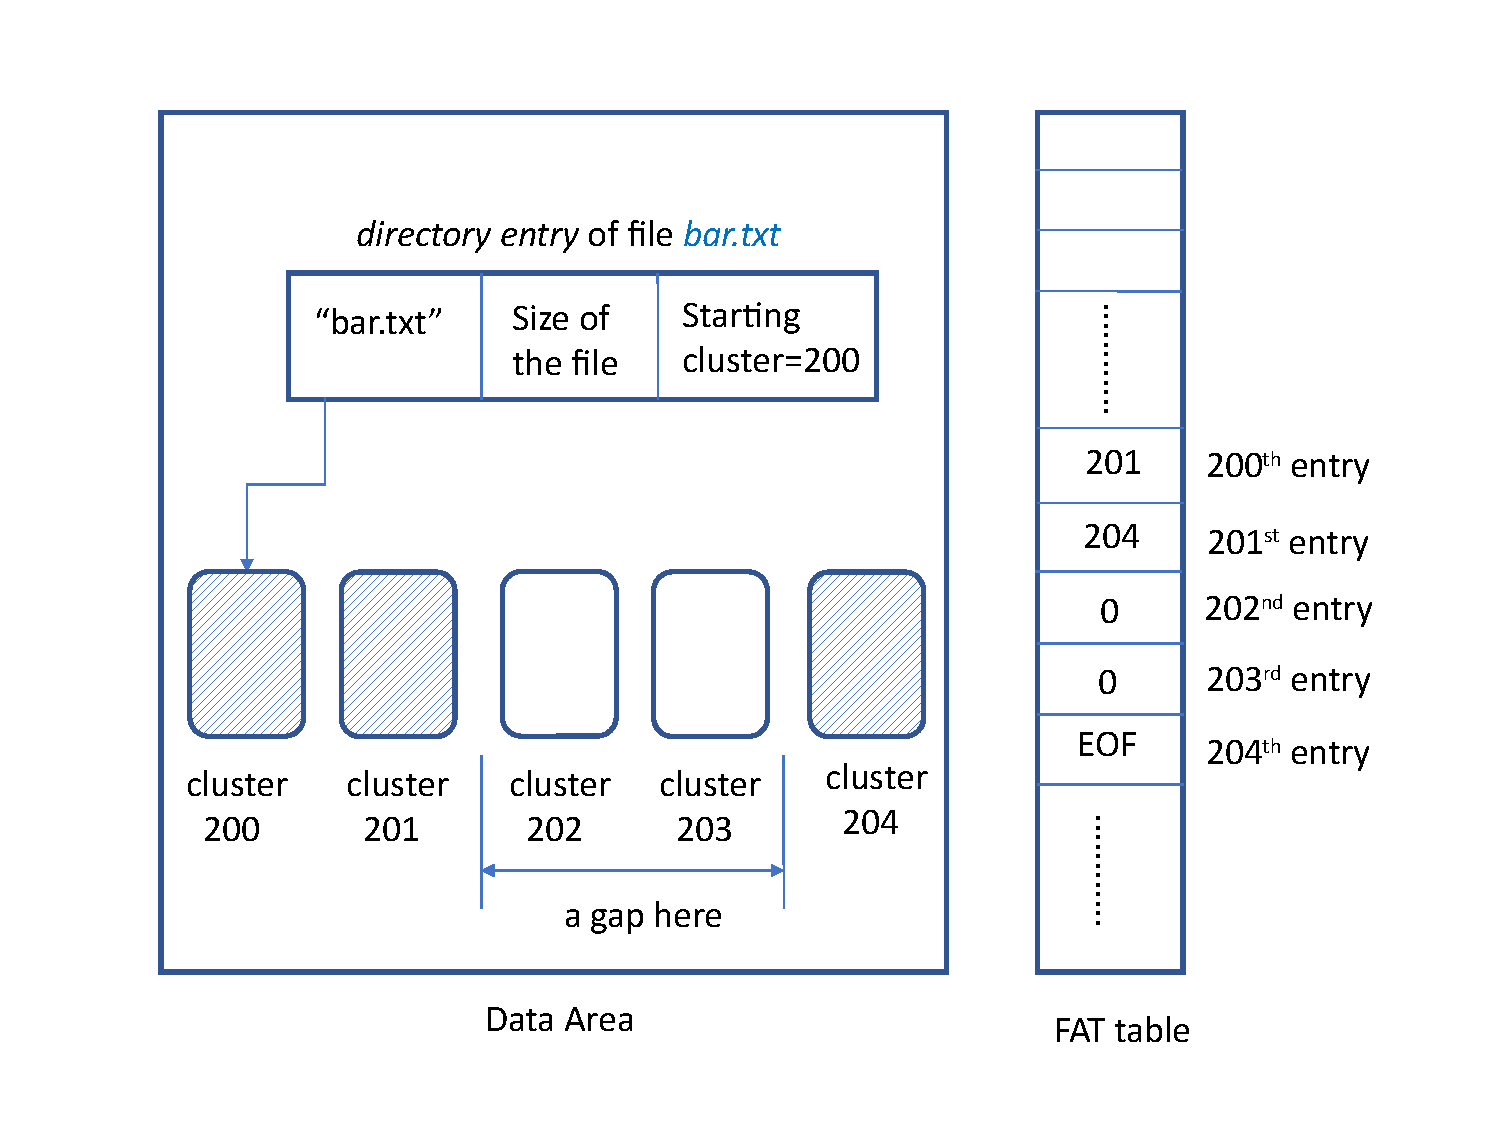
\includegraphics[width=\linewidth]{fig/fat3.pdf}
     \caption{The actual content and metadata of bar.txt is shown. Per the FAT table the file has two fragments (clusters 200-201 and cluster 204).}
     \label{fig:fat3}
 \end{figure}



\subsubsection{NTFS File System} \label{subsubsec:ntfs-overview}

NTFS file system does not maintain a global table (like the FAT table) 
that holds the status for each cluster. Instead NTFS maintains a global table called 
MFT (Master File Table) that
holds information for each file in the system. In particular, each file $f$ has an 
entry in MFT, which holds information about file $f$, and the size of this entry is 1,024 bytes.  
If file $f$ is small, then the whole file content as well as the metadata will be stored
inside $f$'s MFT entry; 
otherwise, $f$'s content is \emph{non-resident} and is stored in other clusters. 
Figure~\ref{fig:ntfs} illustrates an example where the file bar.txt's content is non-resident, 
and it has two fragments. When a file $f$ is deleted in NTFS, 
the corresponding entry in MFT is flagged as deleted and the corresponding clusters 
(if any) are flagged as deleted, but the metadata and file content generally remain intact.
Note that NTFS file system does not have specific zones for data area in contrast of 
FAT having specific area for data and specific area for the FAT table.


 \begin{figure}[h]
     \centering
     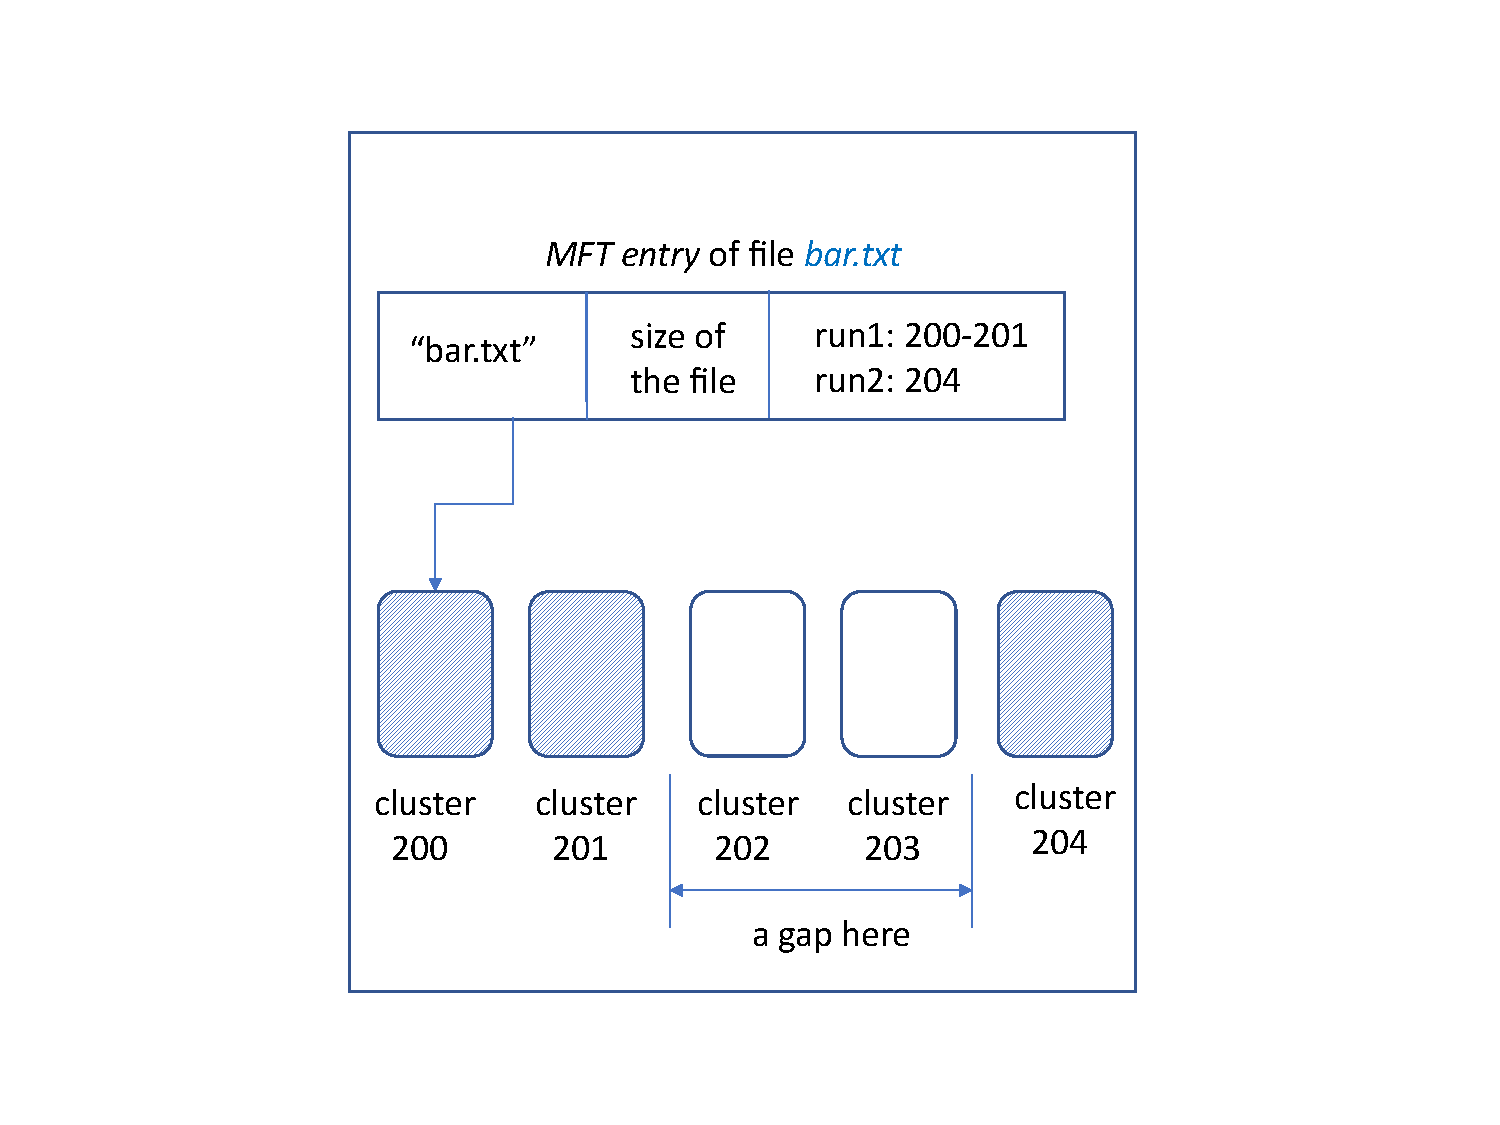
\includegraphics[width=\linewidth]{fig/ntfs.pdf}
     \caption{To illustrate NTFS file system, the MFT entry of bar.txt and the actual content carrying clusters are shown. 
 This file has two fragments (clusters 200-201 and cluster 204).}
     \label{fig:ntfs}
 \end{figure}
 

\subsubsection{Recovering Deleted Files}\label{subsubsec:meta-recovery}

From the previous discussion we note that in many situations the metadata
(e.g., directory entry in FAT or MFT entry in NTFS) of the deleted file remains
unchanged and can be used for identifying and recovering the deleted file.
As an example, the directory entry of bar.txt in Figure~\ref{fig:fat2} tells us
that the file's content starts from cluster $200$, 
and using the \emph{size} field value (e.g., $5$) we can infer that the file's content
is hosted in the cluster chain from cluster $200$ to cluster $204$, assuming that there is no
fragmentation. We can recover the file by reading the raw content of these $5$ clusters, e.g.,
by using \emph{dd} command in Linux.  

We encounter one critical challenge while recovering a fragmented file in FAT because the \emph{directory entry}
of a file does not contain any information about the fragments. However, we do not face this challenge 
in NTFS file recovery because the MFT entry (as shown in Figure~\ref{fig:ntfs}) does contain the start and end cluster index for each run (i.e., fragment). 

\subsection{File Carving}\label{subsec:file-carving}

File carving does not rely on the file system metadata, and hence is independent of the type of the 
file system (e.g., FAT vs. NTFS). In file carving, we assume that the target file has 
a known header and footer signature (i.e., a sequence of special bytes). As an example, 
a JPG file has such a header and a footer signature--in particular, certain two bytes 
for the header and certain two bytes for the footer. The file carving process basically
scans the whole storage space (i.e., the target storage device where we plan to recover deleted files from) 
byte by byte and identifies each match of header and footer signature. 
Then, the content between any header and any footer is potentially a recovered file. 
Depending on the strong vs weak match policy, there could be \emph{false positives} 
(i.e., bogus files being retrieved) 
and \emph{false negatives} (i.e., files missed to be retrieved). 

\subsection{NIST CFTT Guidelines}
NIST CFTT program has published guidelines~\cite{meta:dfr:standards,carving_standards} on how to evaluate deleted file recovery (DFR) tools.

\subsubsection{For Metadata-Based DFR}
NIST's guidelines~\cite{meta:dfr:standards} for evaluating metadata-based DFR tools consist of four \emph{core features} and several \emph{optional features}. We evaluate based only on the core features and leave the optional features for later work.
In this section we list the core features as they appear in the NIST guidelines document, along with our own interpretation and commentary.

 \paragraph{DFR-CR-01} ``The tool shall identify all deleted File System-Object entries accessible in residual metadata''~\cite{meta:dfr:standards}.
 We say a tool fulfills this core feature if it reports something for each file system metadata entry which has been marked as deleted.
 
 \paragraph{DFR-CR-02} ``The tool shall construct a Recovered Object for each deleted File System-Object entry accessible in residual metadata''~\cite{meta:dfr:standards}.
 We say a tool fulfills this core feature if it outputs a file for each of the deleted files identified per DFR-CR-01, even if the output file is empty.

 \paragraph{DFR-CR-03} ``Each Recovered Object shall include all non-allocated data blocks identified in a residual metadata entry''~\cite{meta:dfr:standards}.
 Our interpretation of this feature is file system-dependent as there are differences in what information is available in metadata.
 In the FAT file system, it is impossible to detect fragmentation purely from metadata, so we say a tool fulfills this core feature if it recovers at least all unallocated clusters that were allocated to the first fragment.
 In the NTFS file system, the locations of all fragments are left in metadata after file deletion, so to fulfill this core feature, a tool must recover all unallocated clusters that were allocated to the deleted file.


 \paragraph{DFR-CR-04} ``Each Recovered Object shall consist only of data blocks from the Deleted Block Pool''~\cite{meta:dfr:standards}.
 We say a tool fulfills this core feature as long as the recovered file contains only data from the original deleted file, or null data to represent parts of the file that have been overwritten or are otherwise inaccessible.

\subsubsection{For File Carving} \label{sec:carving_features}

NIST's guidelines~\cite{carving_standards} for evaluating file carving tools consist of five \emph{core features}.
In this section we list the core features as they appear in the NIST guidelines document, along with our own interpretation and commentary.

 \paragraph{FC-CR-01} ``The tool shall return one carved file for each supported file header signature from a source file that is present in the search arena''.~\cite{carving_standards}
 Each file from the original disk will begin with a header signature specific to its file format. We say a tool fulfills this core feature if it carves a file starting at each of those header signatures.
 In other words, tools that perform well on this core feature have a high ``hit rate.''
 
 \paragraph{FC-CR-02} ``A carved file shall only contain data blocks from the search arena''.~\cite{carving_standards}
 In other words, the tool should only work within the drive or partition it is given, and should not try to carve from out-of-bounds.
 
 \paragraph{FC-CR-03} ``All data blocks in a carved file shall originate in a single source file''.~\cite{carving_standards}
 We say a tool fulfills this core feature if each recovered file only contains data from one file on the original disk.
 
 \paragraph{FC-CR-04} ``The file type of a carved file shall match the file type of its contents''.~\cite{carving_standards}
 We interpret this to mean that the file extension given to a recovered file must accurately describe the format of the file data. We exclude false positives from this evaluation because their data is highly unlikely to be of any file format. So, we only consider files which were carved starting from a valid header signature.
 
 \paragraph{FC-CR-05} ``The tool shall return carved files in a state that conforms to a valid file of the carved file type''.~\cite{carving_standards}
 We say a tool fulfills this core feature if each recovered file can be parsed without error by some application software.
 We use the ImageMagick tool suite to evaluate this.

\section{Objectives} \label{rqs}

DFR tools, which come in both metadata-based and file carving variants, are software for recovering deleted data from a digital storage device.
We design experiments to evaluate a selection of DFR tools according to guidelines set by NIST CFTT.
We specifically investigate the following questions:

\begin{itemize}
\item How well do our selected DFR tools meet each of the NIST CFTT guidelines?
\item What conditions influence the success and failure of DFR tools?
\end{itemize}


 

\section{Approach}

To properly evaluate DFR tools, we must see how they perform in various file recovery scenarios.
We do this by running the tools on various \emph{disk images}, each containing a file system with some deleted files.
The recovered files output by a DFR tool are examined to see how well the tool meets the NIST guidelines for deleted file recovery.
By using test images designed to each emphasize specific recovery tasks, we can get a sense of a tools' strengths and weaknesses, and what tasks are especially difficult for certain types of tools.
With this in mind, we designed several disk images to test metadata-based DFR tools.
NIST CFTT has already designed a set of images for testing file carving tools, so we use those rather than creating our own.
A high-level illustration of our methodology can be seen in Figure~\ref{fig:overview}.


\begin{figure}[h]
    \centering
    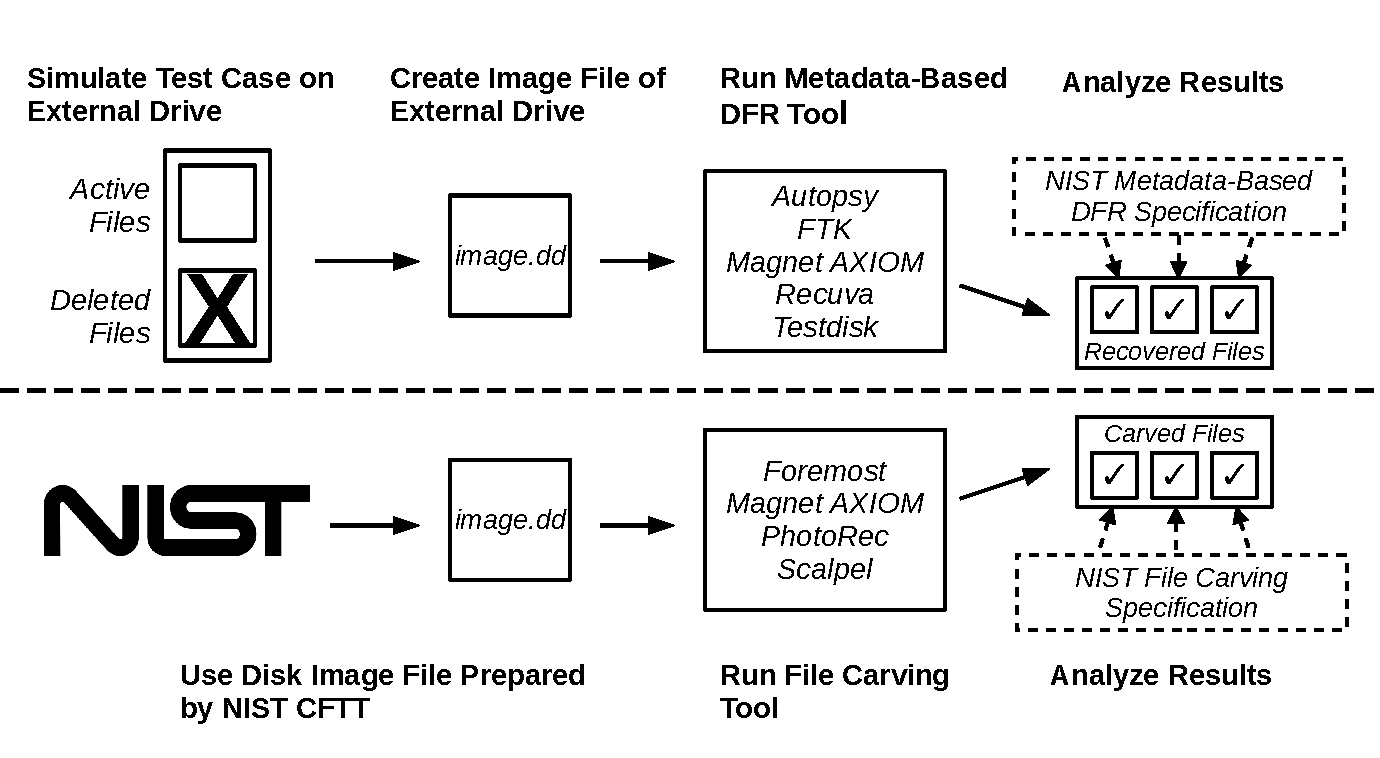
\includegraphics[width=\linewidth]{fig/overview.pdf}
    \caption{
        A read-only \emph{disk image}, a file which contains the raw data of a file system, is obtained for each test case.
        For metadata-based test cases, we create a file system on an external drive and delete files from it, then save it as a disk image.
        For file carving test cases, we use a set of disk images prepared by NIST CFTT.
        In either case disk image is input to a DFR tool, whose output is checked for compliance with the NIST guidelines for metadata-based DFR or file carving, depending on the tool.
    }
    \label{fig:overview}
\end{figure}

\subsection{Metadata-Based Tools}
In this section, we explain our process for testing metadata-based DFR~tools.

\subsubsection{Designing Recovery Scenarios}

We begin by designing a set of test cases to simulate common challenges of metadata-based deleted file recovery.
In order to get the most information possible about each tools' capabilities, we aim to simulate a wide variety of recovery scenarios.
We first isolate the most basic challenges of file recovery, and create test cases for them.
Ideally, these test cases should represent the most basic ``building blocks'' of file recovery scenarios, which can be used to compose more complex scenarios.
When appropriate, we also create test cases representing the basic combinations of these simple cases.
Our intention with this atomic approach is to create test cases that are generalizeable to the majority of recovery scenarios, even the many which we do not explicitly cover.
If a tool performs well on the ``building blocks'' and their basic combinations, we can predict that it will perform similarly on more complex combinations.

In addition to this philosophy, we must remain within the scope of the NIST guidelines.
NIST requires test images to be ``created and deleted in a process similar to how an end-user would create and delete files.''~\cite{meta:dfr:standards}
We take this to mean that any interaction with the file system must be through a standard operating systems'  read and write operations.
We are not allowed to edit the file system directly, as ``files and file system metadata that is specifically corrupted, modified, or otherwise manipulated to appear deleted''~\cite{meta:dfr:standards} are explicitly out of scope.

Within these constraints, we can induce two phenomena which make file recovery more challenging: fragmentation and overwriting.
Following the aforementioned goal of making our tests atomic, all our test cases (besides the first trivial case) use fragmented and/or overwritten files as building blocks.
As such, our test cases fall into five general categories:
{\bf(a)} no fragmentation or overwriting, 
{\bf (b)} only fragmentation,
{\bf (c)} only overwriting,
{\bf (d)} both fragmentation and overwriting,
and {\bf (e)} fragmentation ``out of~order.''


Each test case is listed in Table~\ref{meta_cases} along with a brief description.
We have given each a distinct name in line with the naming scheme for the CFTT file carving test cases.
A selection of test cases are illustrated, with each column in an illustration portraying the state of the file system at a point in time. 
Each file is given a unique letter and shading, and the start and end of a fragmented file are denoted when relevant.

\begin{table}[ht!]
\tbl{Metadata-based DFR test cases}
{\begin{tabular*}{\textwidth}{@{}rp{0.8\linewidth}@{}} \toprule
\multicolumn{2}{c}{\textbf{Basic Deleted File}} \\ \colrule
\textbf{basic} & Deleted file is contiguous and the only file on the disk \\
\colrule
\multicolumn{2}{c}{\textbf{Deleted File is Fragmented}} \\ \colrule
\textbf{fragments1} & Deleted file is fragmented around an active file (illustrated in Figure~\ref{fig:case2}) \\
\textbf{fragments2} & Deleted file is fragmented around another deleted file \\
\colrule
\multicolumn{2}{c}{\textbf{Deleted File is Overwritten}} \\ \colrule
\textbf{overwrite1} & Deleted file is overwritten at the front by an active file \\
\textbf{overwrite2} & Deleted file is overwritten in the middle by an active file (illustrated in Figure~\ref{fig:case5}) \\
\textbf{overwrite3} & Deleted file is completely overwritten by an active file \\
\textbf{overwrite4} & Deleted file is overwritten at the front by another deleted file (illustrated in Figure~\ref{fig:case8}) \\
\textbf{overwrite5} & Deleted file is overwritten in the middle by another deleted file \\
\textbf{overwrite6} & Deleted file completely overwritten by another deleted file \\
\colrule
\multicolumn{2}{c}{\textbf{Deleted File is Fragmented and Overwritten}} \\ \colrule
\textbf{combo1} & Deleted file is fragmented around an active file, and the second fragment is overwritten by another active file (illustrated in Figure~\ref{fig:case12}) \\
\textbf{combo2} & Deleted file is fragmented around an active file, and the second fragment is overwritten by another deleted file \\
\colrule
\multicolumn{2}{c}{\textbf{Deleted File is Fragmented Out-of-Order}} \\ \colrule
\textbf{disorder1} & Deleted file fragmented out-of-order with empty space in between the fragments (illustrated in Figure~\ref{fig:case14}) \\
\textbf{disorder2} & Deleted file fragmented out-of-order with an active file in between the fragments \\
\textbf{disorder3} & Deleted file fragmented out-of-order with a deleted file in between the fragments \\
\botrule
\end{tabular*}}
\label{meta_cases}
\end{table}


\begin{figure}
    \centering
    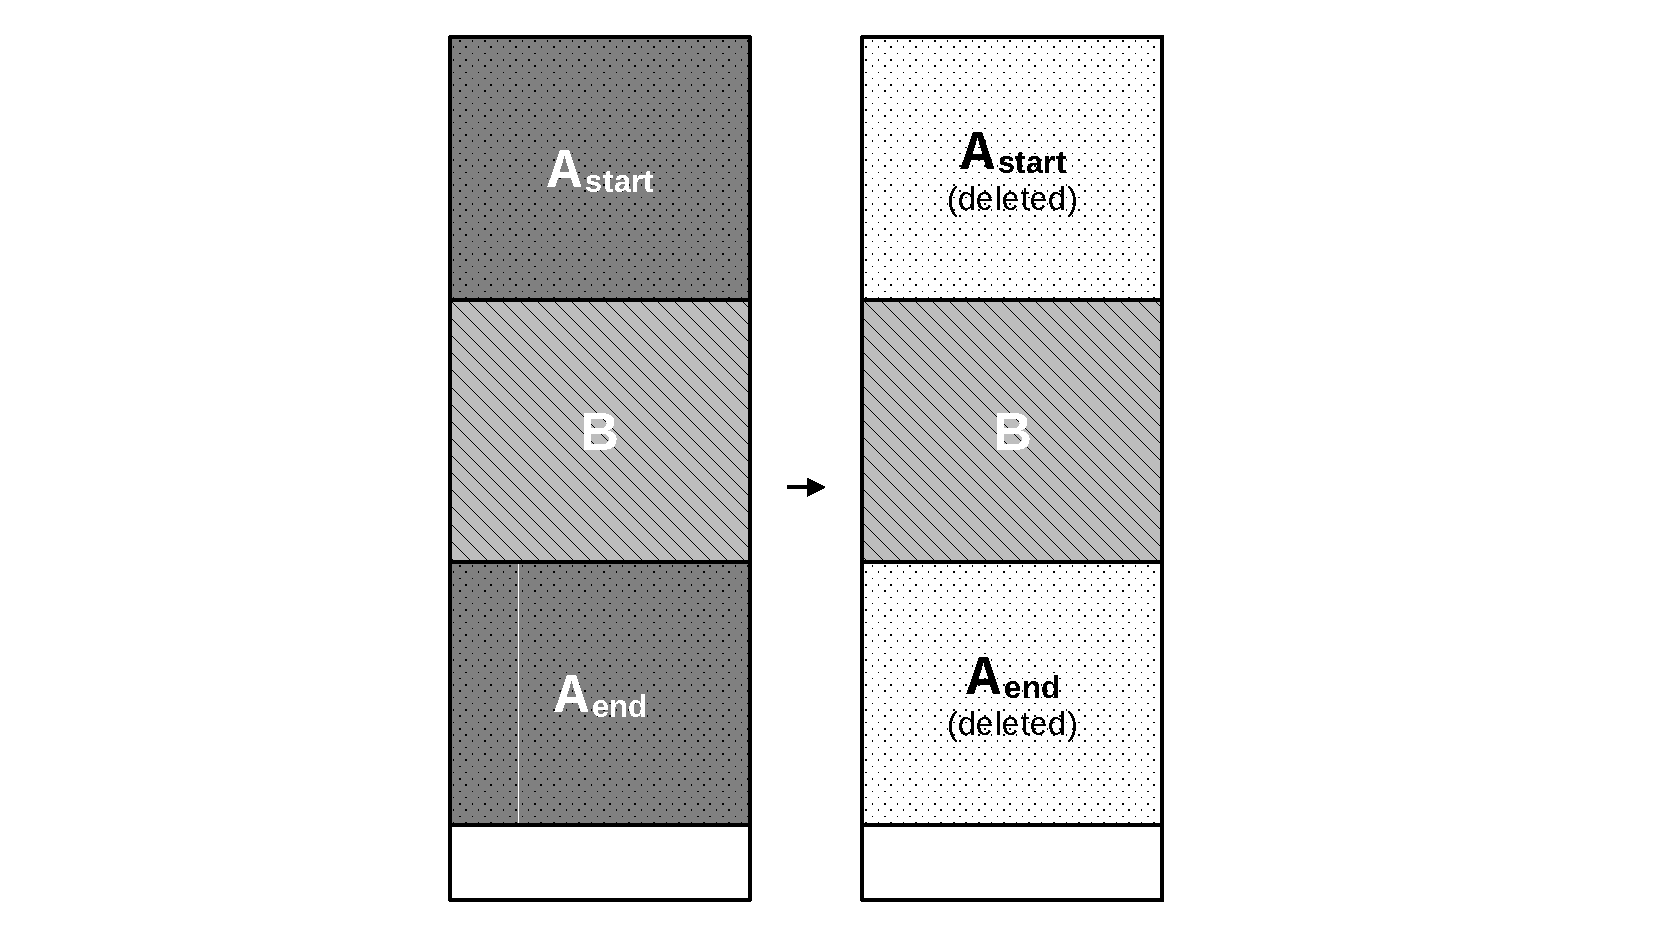
\includegraphics[width=\linewidth]{fig/case2.pdf}
    \caption{fragments1: File A is fragmented and has been deleted.}
    \label{fig:case2}
\end{figure}

\begin{figure}
    \centering
    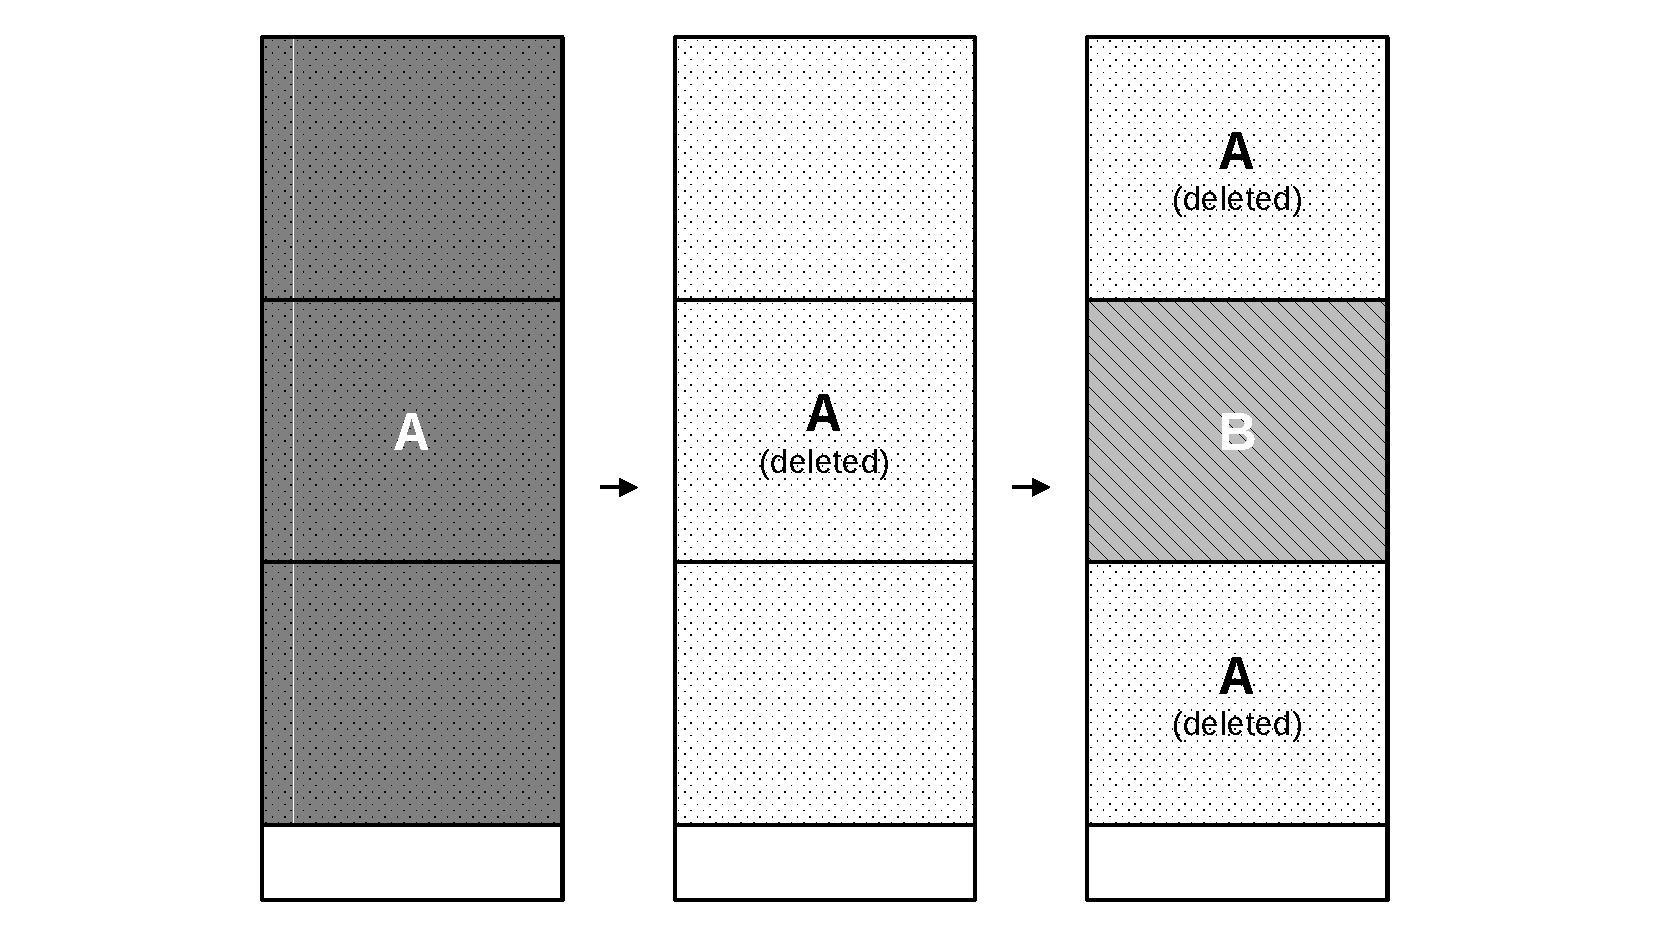
\includegraphics[width=\linewidth]{fig/case5.pdf}
    \caption{overwrite1: File A has been deleted and partially overwritten by file B.}
    \label{fig:case5}
\end{figure}

\begin{figure}[h]
    \centering
    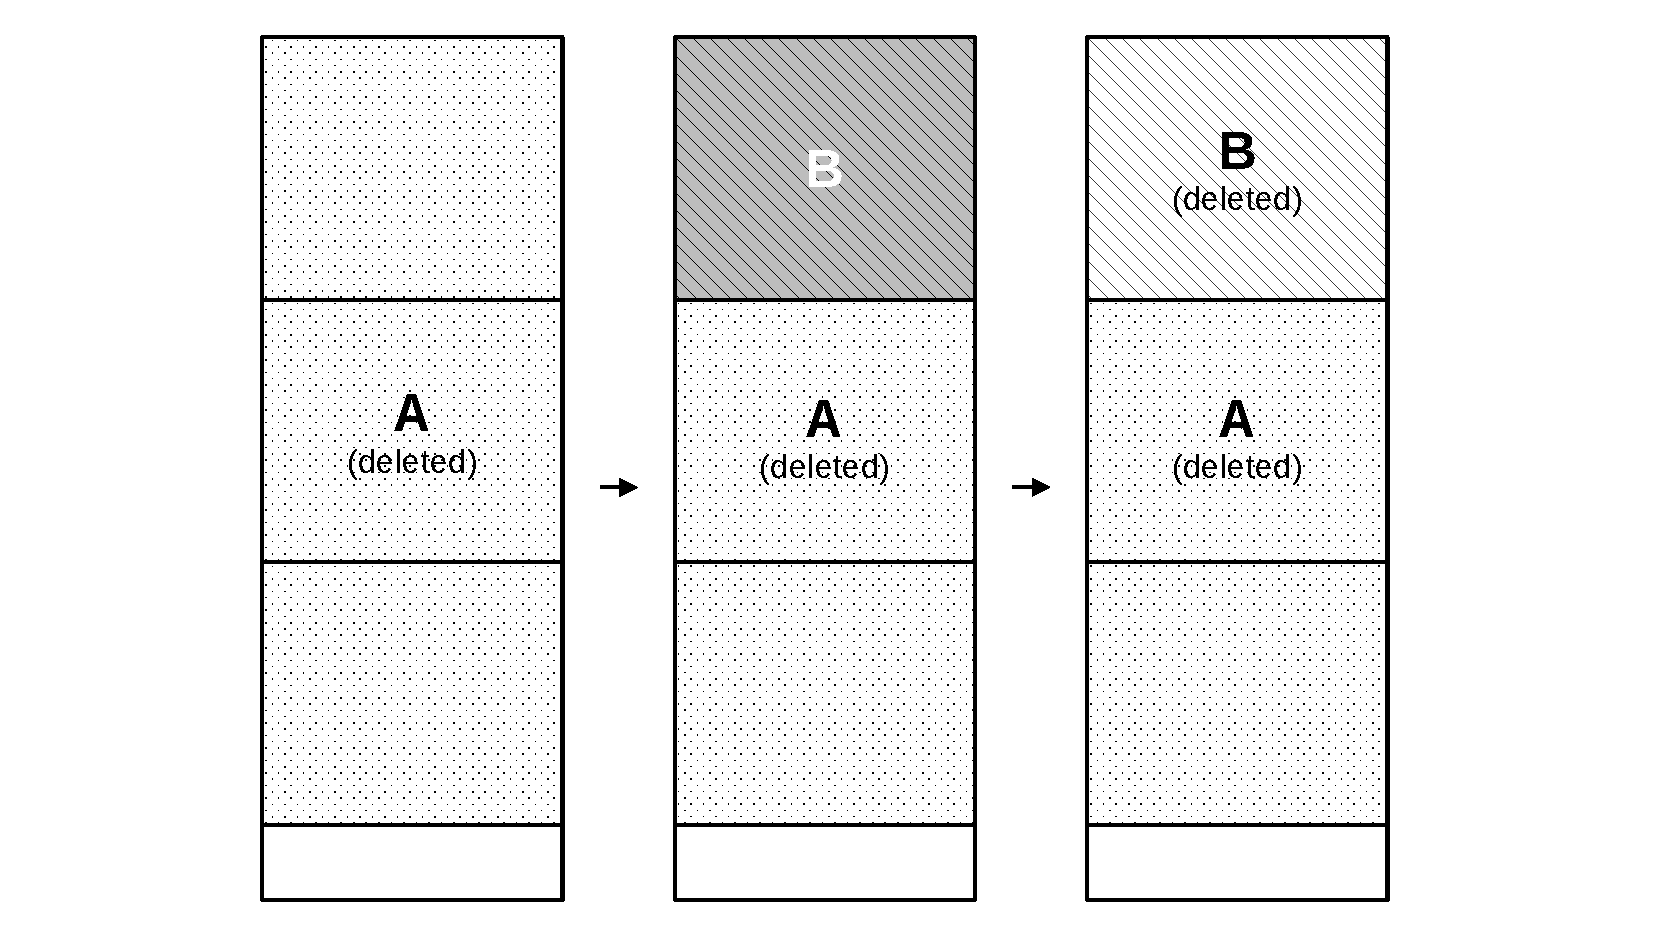
\includegraphics[width=\linewidth]{fig/case8.pdf}
    \caption{overwrite4: File A has been deleted and partially overwritten by file B, which has since been deleted.}
    \label{fig:case8}
\end{figure}

\begin{figure}[h]
    \centering
    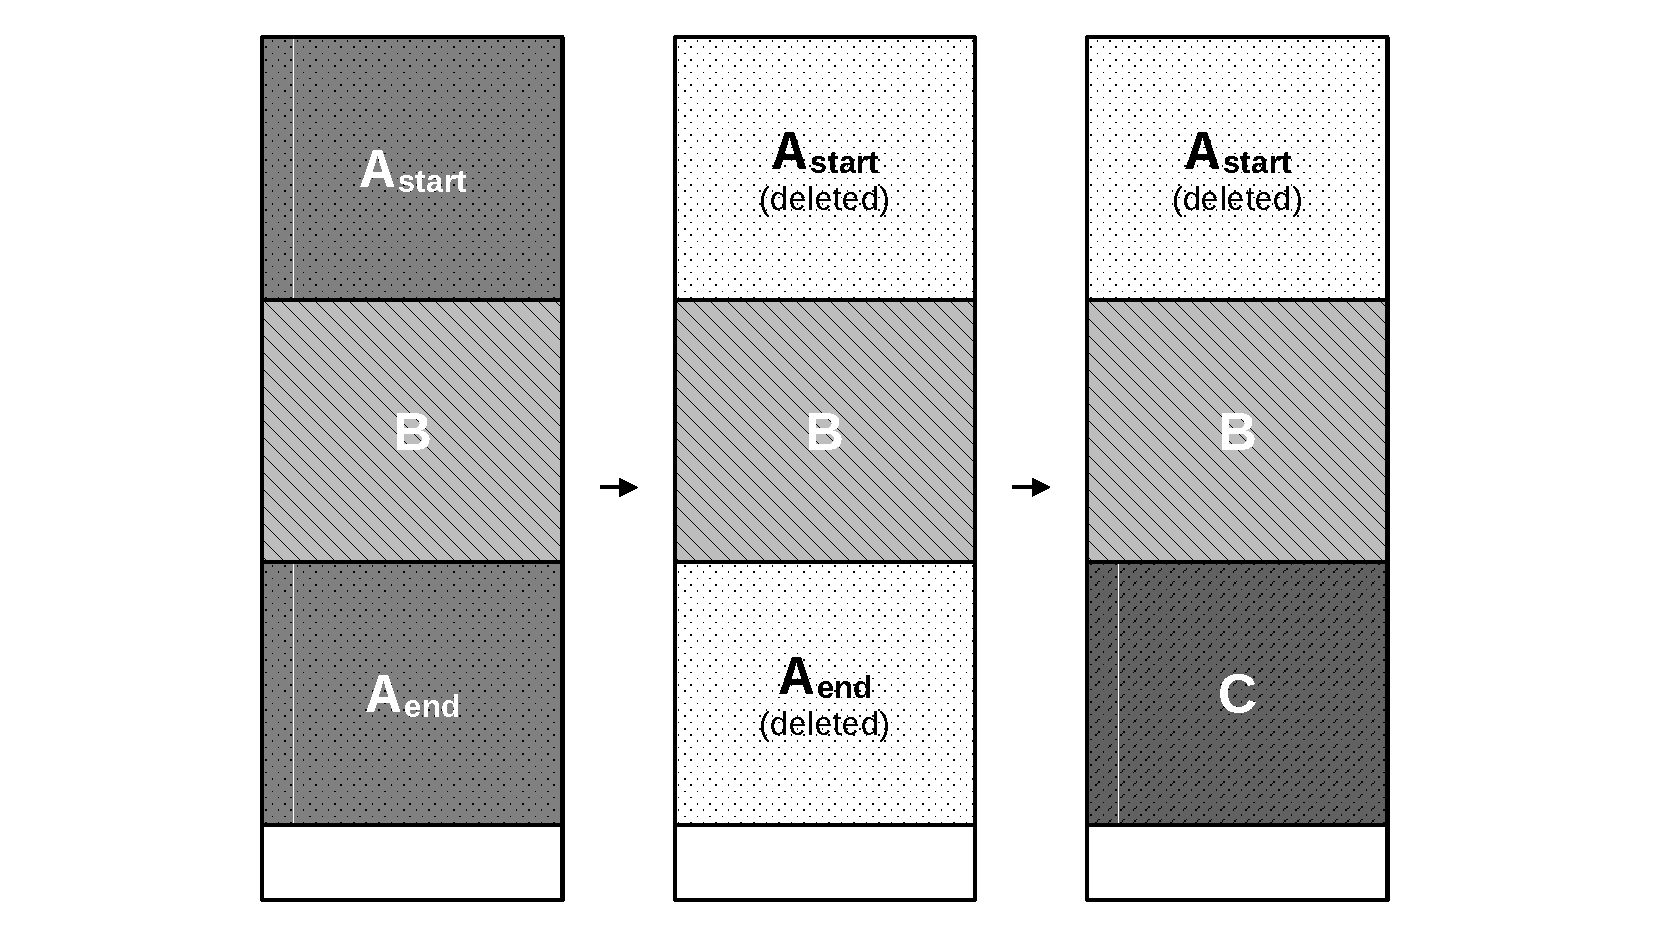
\includegraphics[width=\linewidth]{fig/case12.pdf}
    \caption{combo1: File A is fragmented and has been deleted. The second fragment has then been overwritten by file C.}
    \label{fig:case12}
\end{figure}

\begin{figure}[h]
        \centering
        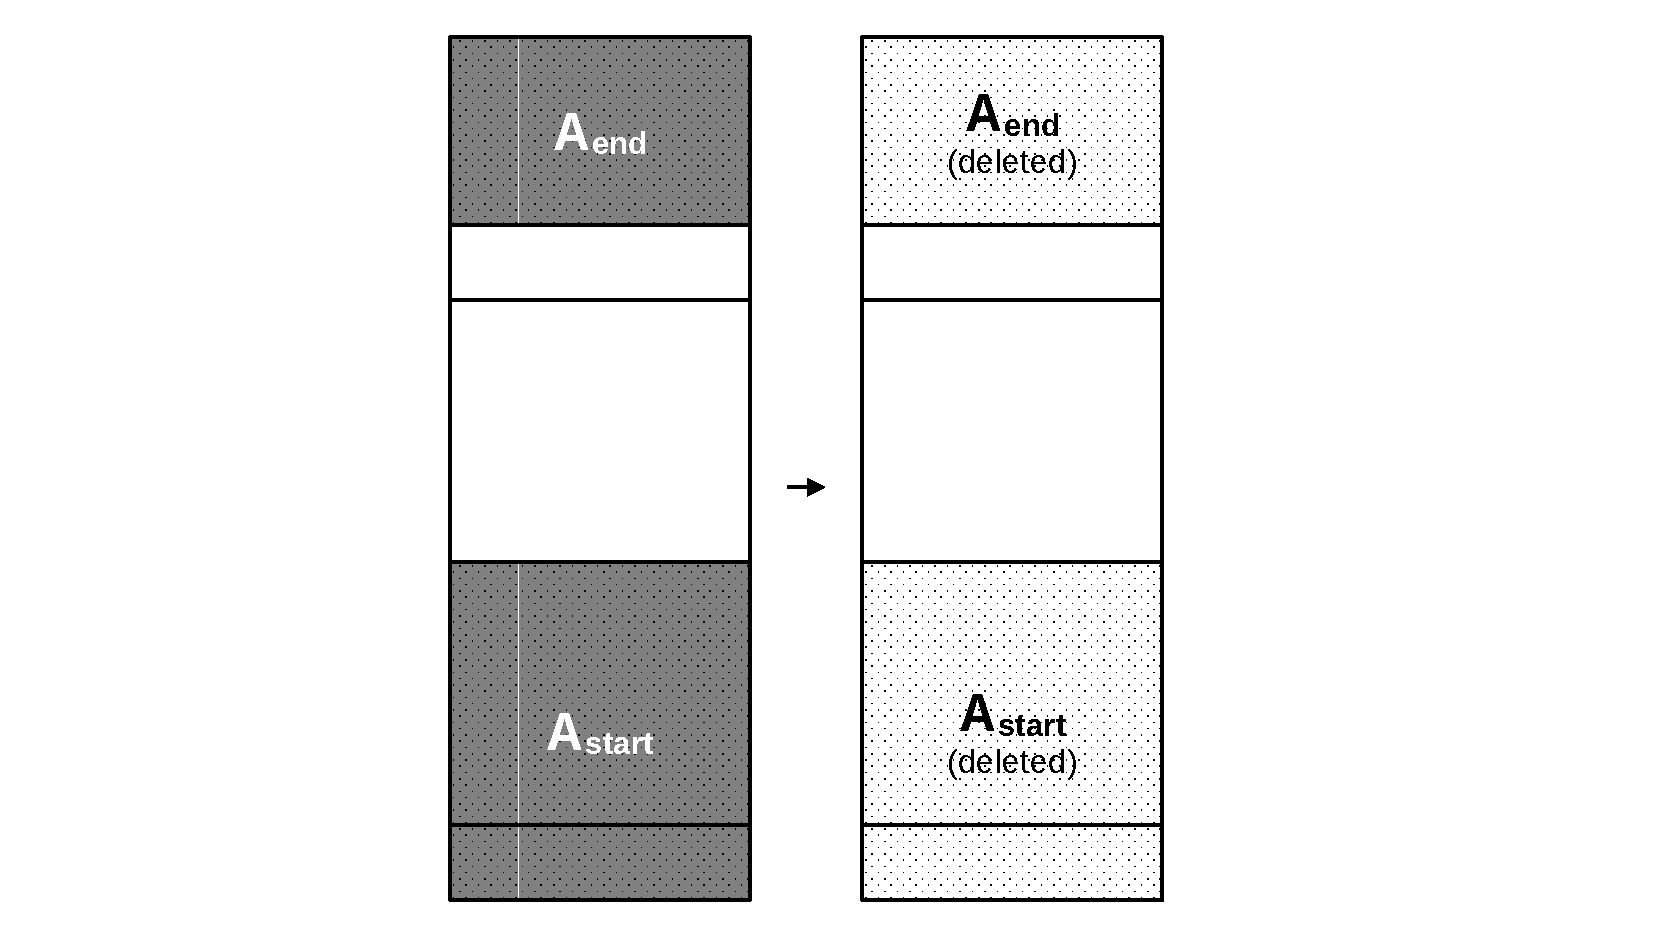
\includegraphics[width=\linewidth]{fig/case14.pdf}
        \caption{disorder1: File A is fragmented out-of-order, and has been deleted.}
        \label{fig:case14}
\end{figure}


Fragmentation is trivial in NTFS because information about the runs of a file persist after deletion.
Since this renders the \emph{fragments} and \emph{disorder} cases functionally identical, we test only the \emph{fragments} cases for NTFS.
Cases \emph{overwrite2} and \emph{overwrite5} cannot be created through regular file operations in NTFS, due to NTFS's file allocation behavior.
Thus, we also exclude \emph{overwrite2} and \emph{overwrite5} for NTFS.
We do not exclude any test cases when using FAT.


\subsubsection{Creating Test Images}

We create the test cases on a 32 GB flash drive, using 4 MiB partitions for FAT cases and 6 MiB partitions for NTFS cases.
For each case, it is important to start by writing over the partition with zeroes, ensuring the image is easily reproducible.
Next, a file system should be written to the partition, and files should be written to it and deleted until the file system matches one of the planned test cases.
We used text files, each containing a single repeated letter (e.g., ``aa1M'' is a text file containing 1 MiB of the letter `a')
Note that text files cannot be recovered with file carving, so this choice forces tools which combine both DFR methods to rely solely on metadata-based recovery.
We write files to the test file system by copying them from another drive, and appending to files when we need to force fragmentation.
Once the test file system matches one of the planned test cases, we use the \emph{dd} utility to create a disk image of that partition.
Since the disk image can be made read-only, it is safer and more convenient to run tests on the disk image instead of the physical drive.
Note that we create FAT test cases using Ubuntu 18.04 and NTFS test cases using Windows~10.

\subsubsection{Challenges}

 % Caching problem
Creating test images can be difficult without a solid understanding of low-level file system behavior.
For example, a newly written file may not have its data written to the disk right away.
Even with fast modern storage, disk I/O involves a considerable amount of overhead.
To improve performance, operating systems generally prefer to write data in one larger batch versus several small batches.
So, the operating system will often store write operations in a cache and wait for a more optimal moment to actually write to the disk.
Typically, this optimization only causes problems in the event of sudden power loss or improper shutdown, but it can also make the state of the file system less predictable.
We found that we were often deleting a file while it was still cached, meaning it would never be written to the disk to begin with.
This is obviously a problem as it leaves nothing on the disk to recover.
Thankfully, Linux and Windows both provide a \emph{sync} system call, which causes the cached writes to be performed immediately.
Calling sync before each file deletion resolves the issue; alternatively, unmounting the file system triggers similar behavior.

% Learning and using the allocation algorithms
Since most of the test images involve manipulating file data into certain arrangements, it is also helpful to have some understanding of allocation algorithms.
Allocation algorithm refers to the steps the operating system takes to decide where on the disk to write new data.
Generally, the operating system wants to limit fragmentation, as contiguous files are more efficient to read and write to.
Common allocation algorithms like ``first available,'' ``next available,'' and ``best fit'' will place files according to that general principle, but use differing strategies to do so.

Understanding the allocation algorithm removes a lot of trial and error from the process of making test images.
For example, we observed that Linux uses a ``next available'' algorithm when writing to FAT.
After mounting the file system, the first file to be written will be placed at the first available space in the file system.
However, unlike the ``first available'' algorithm, the operating system remembers where it last placed a file, and it will place the next file at the first available space after that saved location, even if space opens up at the beginning of the file system.
Windows, on the other hand, uses a ``best fit'' algorithm when writing to NTFS.
This allocation algorithm takes a more proactive approach to reducing fragmentation by writing each file to the smallest space in which it can fit without being fragmented.


\subsubsection{Recovering Files}

We chose to test five popular DFR tools: Autopsy~\cite{autopsy}, FTK Imager~\cite{ftk}, Magnet AXIOM~\cite{axiom_meta}, Recuva~\cite{recuva}, and TestDisk~\cite{testdisk}.
For Autopsy, we performed a standard recovery with ingest modules disabled.
For FTK Imager, we used the free version and performed a standard recovery with default settings.
For Magnet AXIOM we used AXIOM Process to perform a ``full scan'', then exported all files accessible from ``Filesystem View'' in AXIOM Examine.
For Recuva we used the free version to perform a standard recovery with default settings.
For TestDisk we used ``file undelete'' in ``Advanced Filesystem Utils'' to recover files.

\subsubsection{Results}

\begin{figure}
    \centering

    \begin{subfigure}{0.3\linewidth}
        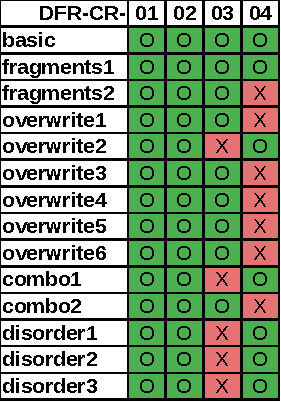
\includegraphics[width=\linewidth]{fig/autopsy_results_fat.pdf}
        \subcaption{Autopsy}
    \end{subfigure}~~
    \begin{subfigure}{0.3\linewidth}
        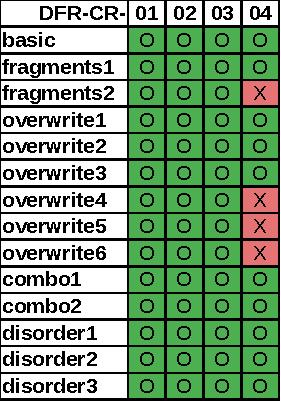
\includegraphics[width=\linewidth]{fig/ftk_results_fat.pdf}
        \subcaption{FTK}
    \end{subfigure}
    \begin{subfigure}{0.3\linewidth}
        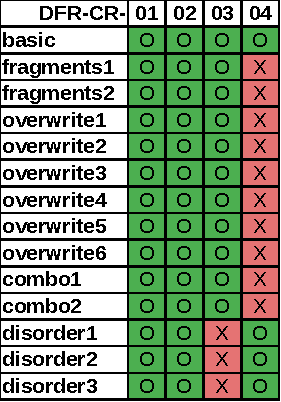
\includegraphics[width=\linewidth]{fig/axiom_results_fat.pdf}
        \subcaption{Magnet AXIOM}
    \end{subfigure}~~
    \begin{subfigure}{0.3\linewidth}
        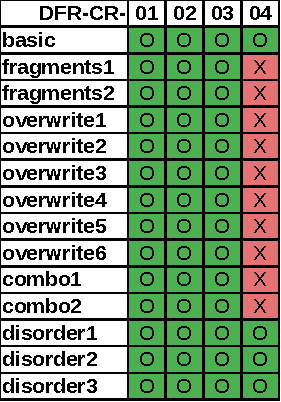
\includegraphics[width=\linewidth]{fig/recuva_results_fat.pdf}
        \subcaption{Recuva}
    \end{subfigure}~~
    \begin{subfigure}{0.3\linewidth}
        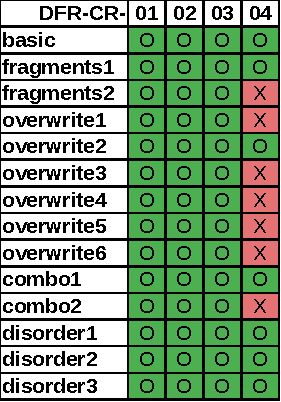
\includegraphics[width=\linewidth]{fig/testdisk_results_fat.pdf}
        \subcaption{TestDisk}
    \end{subfigure}
        
    \caption{Test results on metadata-based DFR tools using FAT-formatted test images. Each row corresponds to a test image and each column corresponds to a core feature. An ``O'' indicates success and an ``X'' indicates failure.}
    \label{fig:results_fat}
\end{figure}

\begin{figure}
    \centering

    \begin{subfigure}{0.3\linewidth}
        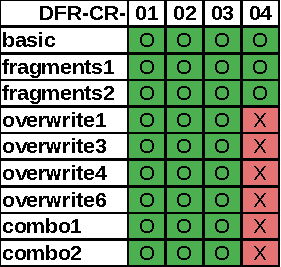
\includegraphics[width=\linewidth]{fig/autopsy_results_ntfs.pdf}
        \subcaption{Autopsy}
    \end{subfigure}~~
    \begin{subfigure}{0.3\linewidth}
        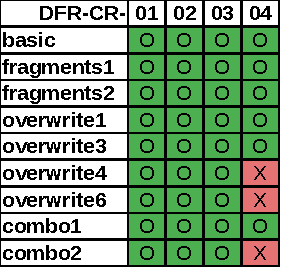
\includegraphics[width=\linewidth]{fig/ftk_results_ntfs.pdf}
        \subcaption{FTK}
    \end{subfigure}
    \begin{subfigure}{0.3\linewidth}
        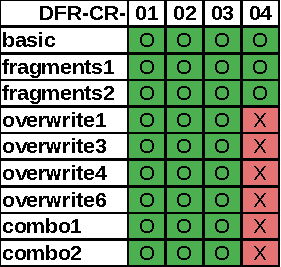
\includegraphics[width=\linewidth]{fig/axiom_results_ntfs.pdf}
        \subcaption{Magnet AXIOM}
    \end{subfigure}~~
    \begin{subfigure}{0.3\linewidth}
        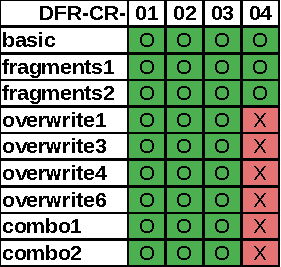
\includegraphics[width=\linewidth]{fig/recuva_results_ntfs.pdf}
        \subcaption{Recuva}
    \end{subfigure}~~
    \begin{subfigure}{0.3\linewidth}
        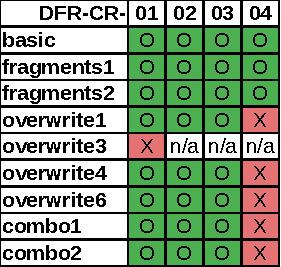
\includegraphics[width=\linewidth]{fig/testdisk_results_ntfs.pdf}
        \subcaption{TestDisk}
    \end{subfigure}
        
    \caption{Test results on metadata-based DFR tools using NTFS-formatted test images. Each row corresponds to a test image and each column corresponds to a core feature. An ``O'' indicates success, an ``X'' indicates failure, and a ``n/a'' indicates no judgement could be made.}
    \label{fig:results_ntfs}
\end{figure}


After running a DFR tool for a test case, we examine the files output by the tool to see if the NIST guidelines have been met.
Note that a file does not need to be perfectly recovered for a tool to meet the guidelines, although all the guidelines would be met in that case.
Sometimes, as with overwritten files, part of the file's data literally no longer exists on the disk, so recovering the entire file is impossible.
The NIST guidelines are designed with this reality in mind.

Most tools recover files perfectly for FAT \emph{fragments1}, and all tools recover files perfectly for FAT \emph{basic}, NTFS \emph{basic}, and NTFS \emph{fragments1} and \emph{fragments2}.
For the other cases, we need to examine the recovered files closely to see which core features are being met.
We judge each tool as either meeting or failing each core feature individually for each test case.
Results are shown in Figure~\ref{fig:results_fat} and Figure~\ref{fig:results_ntfs} for FAT and NTFS test cases, respectively.

Note that in the one test case where DFR-CR-01 is not met, meaning no deleted file was detected, we cannot make a judgement for the other core features.



\paragraph{Recovering Fragmented Files}
We observe that tools typically use one of two strategies in the event of FAT fragmentation.
The first is to simply ignore fragmentation and recover the full length of a file as though it is contiguous, even if there are active files in that length.
Recuva and Magnet AXIOM seem to take this approach.
The second strategy is to still recover the full length of the file, but only from unallocated space.
So, any active files will be skipped over.
Autopsy, FTK, and TestDisk seem to take this approach.
This is most easily observed in FAT \emph{fragments1}; Autopsy, FTK, and TestDisk will skip over file B to recover all of file A, while Recuva and Magnet AXIOM will recover the first fragment of file A along with the active file B.
This is why Recuva and Magnet AXIOM fail DFR-CR-04 for that case.
However, when a file is fragmented around another deleted file, like in FAT \emph{fragments2}, all tools take the first approach and erroneously return file B as part of file A.
All tools seem to struggle with out-of-order fragmentation.
When the first fragment is at the very end of the file system, Recuva, FTK, and TestDisk only recover the first fragment, Autopsy returns a small amount of null data, and Magnet AXIOM returns an empty file and an error message.

In NTFS more information about a file's location remains after the file is deleted, so recovering fragmented files is trivial.
All tools we tested are able to handle fragmentation in NTFS with no issues.


\paragraph{Recovering Overwritten Files}
We observe that when a deleted file is overwritten by an active file, most tools still attempt to recover the overwritten part as though it was part of the original file, failing DFR-CR-04.
The only tool to consistently meet DFR-CR-04 in these cases is FTK Imager, which only recovers data from before the overwritten part.
TestDisk also does this for FAT \emph{overwrite2} only, otherwise behaving like the other tools.
In FAT, Autopsy only recovers the first cluster of an overwritten file, regardless of what part was overwritten.
In NTFS, it gives the same results as other tools.
For FAT \emph{overwrite1} and \emph{overwrite2}, Magnet AXIOM recovers up to the end overwritten sections, but no further.
This is a bit strange as it suggests Magnet AXIOM can detect overwriting, but still returns the overwritten part.
For other cases, it behaves like the other~tools.

When a deleted file is overwritten by another deleted file, even FTK acts as though the overwritten part belongs to the original file.
This suggests that the tools which can detect overwriting do so based on the allocation status of each data block; other than that, they only consider the metadata of the file being recovered, not the files around it.

\paragraph{Miscellaneous}
Several FAT test cases (\emph{overwrite2}, \emph{combo1}, \emph{disorder1}, \emph{disorder2}, and \emph{disorder3}) cause Autopsy to return a 1.5 KiB file containing null data.
This is particularly odd because a FAT cluster is 2 KiB; making these the only recovered objects not divisible into clusters.
Given the odd size and contents, we suspect this is some sort of error state rather than an attempted recovered file.

TestDisk does not identify any deleted file in NTFS \emph{overwrite3}.
While the deleted file's data is entirely overwritten in this case, information about the file is still present in metadata.
Since this only happens in NTFS and not FAT, meaning the precise location of the deleted file is still available, it is possible that TestDisk is able to detect the fact that the file has been overwritten, and simply ignores it.
Even if this is the case, the file information is still available in metadata, so the for TestDisk to meet DFR-CR-01, it must identify the file regardless of whether it can be recovered.


\subsection{Carving-Based Tools}
In this section, we explain our process for testing file carving-based DFR~tools.

\subsubsection{CFTT Test Cases}
To evaluate the file carving tools, we used six disk images prepared by CFTT~\cite{cftt_carving_images}.
Each of these images contains between 20 and 40 graphical files of the JPG, PNG, GIF, BMP, and TIFF formats.
Importantly, the CFTT images do not contain valid file systems.
This ensures that a tool which utilizes both DFR methods can be evaluated solely on its file carving ability.

Despite the differences between the methods, metadata-based DFR and file carving are complicated by the same two file system behaviors: fragmentation and overwriting. Thus, the CFTT test cases are somewhat similar to the ones we created for metadata-based DFR; each is built around a specific variation of fragmentation or overwriting of deleted files.
Summaries of each CFTT test image are given in Table~\ref{carve_cases}.

\begin{table}[ht!]
\tbl{File carving test cases}
{\begin{tabular*}{\textwidth}{@{}rp{0.8\linewidth}@{}} \toprule
\textbf{basic} & 40 contiguous files, with space in between each file \\
\textbf{nofill} & 40 contiguous files, with no space in between each file \\
\textbf{simple-frag} & 40 fragmented files, with space in between each fragment \\
\textbf{braid} & 10 contiguous files and 10 fragmented files, which are fragmented around each other in an A-B-A-B pattern \\
\textbf{disorder} & 35 fragmented files, 30 of which are fragmented out-of-order such that the fragment containing the footer comes before the fragment containing the header \\
\textbf{partials} & 15 complete files, 5 of which are fragmented, and 25 incomplete files where at least one fragment has been overwritten or manually destroyed \\
\botrule
\end{tabular*}}
\label{carve_cases}
\end{table}


\subsubsection{Recovering Files}

We chose to test four popular file carving tools: PhotoRec~\cite{photorec}, Foremost~\cite{foremost}, Scalpel~\cite{scalpel}, and Magnet AXIOM~\cite{axiom_carve}.
Note that since tests were run at different times, the version of Magnet AXIOM used for carving tests is newer than the version used for metadata-based tests.

The settings we used when testing each tool are as follows:
For PhotoRec and Foremost, we used the default settings.
For Scalpel, we manually enabled recovery of the JPG, PNG, GIF, BMP, and TIFF formats, and otherwise used default settings.
For Magnet Axiom, we ran a ``sector-level scan'' with default settings in AXIOM Process and exported all graphical files from ``Artifact View'' in AXIOM Examine.
We also exported an XML carving report from Axiom Examine as unlike the other tools it does not create one automatically.

\subsubsection{Evaluating Results}
The main challenge when testing file carving tools is verifying the results. 
For metadata-based tools this is fairly simple; the deleted files in our tests are all simple text files which can be checked at a glance.
However, text files lack a standard header and footer and thus cannot be recovered with file carving, so the test images use more complicated formats such as JPG.
As a result, it would be impractical to evaluate a tool based on the carved files alone.

Fortunately, all four of the carving tools we evaluated produce an itemized report of carving results. CFTT provides detailed information about the contents of the test images, so we can compare the tools' reports with the true arrangement of files in each image. This is particularly important for FC-CR-01, FC-CR-02, and FC-CR-03 since they are concerned with the specific data blocks the tool carves. PhotoRec's report gives a start and end address for each file, and multiple start and end addresses if it attempts to carve a fragmented file. The other tools' reports only list the starting address and size of each file, so we assumed they never attempt to carve more than one fragment per file.

Checking FC-CR-04 is slightly complicated by the fact that carving tools cannot recover the filename, but we can use the first sector listed for each file in the carving report to match them with the original files and check the file extensions.

For FC-CR-05, we make use of the \emph{identify} command from the ImageMagick~\cite{imagemagick} tool suite. Upon input of a graphical file, identify will output the file format and other information. Relevant to FC-CR-05 is that the return code will indicate whether the file is valid or corrupt. We add the \emph{-regard-warnings} flag so an error or warning while parsing the file will mean the file is considered corrupt.

\subsubsection{Results}

\begin{figure}
    \centering

    \begin{subfigure}{\linewidth}
        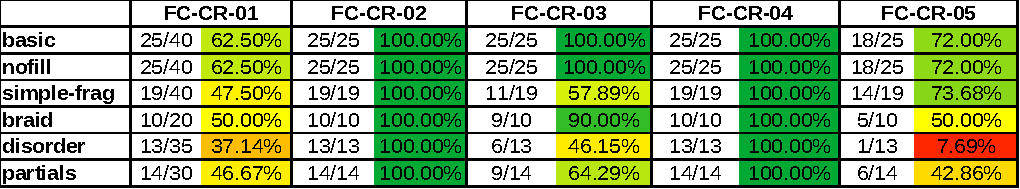
\includegraphics[width=\linewidth]{fig/foremost_results_carve.pdf}
        \subcaption{Foremost}
    \end{subfigure}
    \begin{subfigure}{\linewidth}
        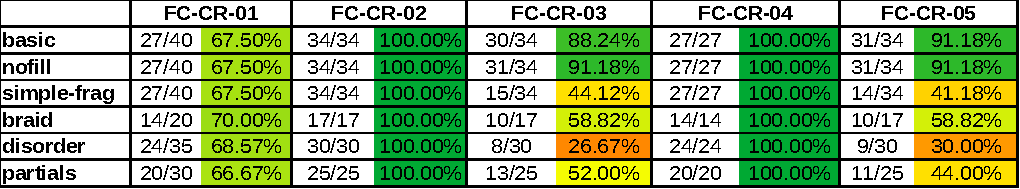
\includegraphics[width=\linewidth]{fig/axiom_results_carve.pdf}
        \subcaption{Magnet AXIOM}
    \end{subfigure}
    \begin{subfigure}{\linewidth}
        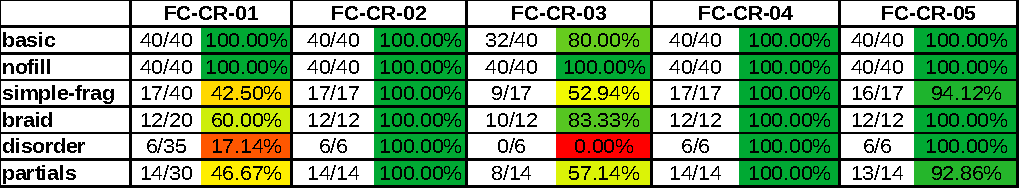
\includegraphics[width=\linewidth]{fig/photorec_results_carve.pdf}
        \subcaption{PhotoRec}
    \end{subfigure}
    \begin{subfigure}{\linewidth}
        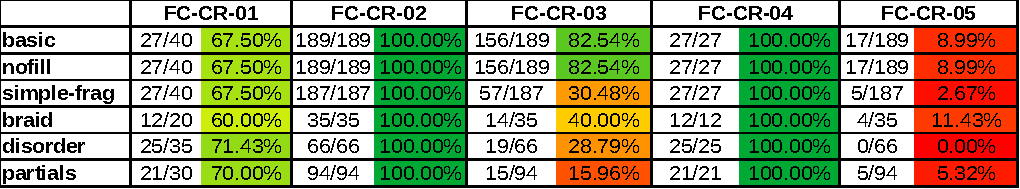
\includegraphics[width=\linewidth]{fig/scalpel_results_carve.pdf}
        \subcaption{Scalpel}
    \end{subfigure}
        
    \caption{
    Results from testing file carving tools. 
    Each row represents a test case, and each column represents a core feature. 
    Since each test image contains many files, we score a tool's compliance with the NIST guidelines by determining the percentage of files for which each core feature is met.
    In each case, scores are given in both fractional and percent form.
    %For details on how the numbers are determined, see the explanation of core features in Section~\ref{sec:carving_features}.
    }
    \label{fig:results_carve}
\end{figure}

% CR1: hit rate, hits/source files
% CR2: in-bounds/carved, trivial
% CR3: one-source/carved, often still a valid file
% CR4: hits identified correctly/hits, trivial
% CR5: valid/carved, 

%Results for file carving tools can be seen in Figure~\ref{fig:results_carve}.

For FC-CR-01, Scalpel and Magnet AXIOM score between 60\% and 70\% for all test cases, Foremost scores between 37\% and 63\%, and PhotoRec ranges from a perfect score to as low as 17\% depending on the test case.
A high score on this core feature means a tool detects most of the original deleted files in a given test case, in other words, it has a high ``hit rate.''

All tools perfectly fulfill FC-CR-02, meaning they never try to carve data from outside the drive or partition given as input.

For FC-CR-03, each tool achieves high scores on some test cases and low score on others.
A high score on this core feature means most of the files a tool recovers contain data from only one other source.
Note that carving from multiple sources may still result in a valid file, such as in Figure~\ref{fig:CR3_fail}.

\begin{figure}
    \centering
    \begin{subfigure}{0.45\linewidth}
        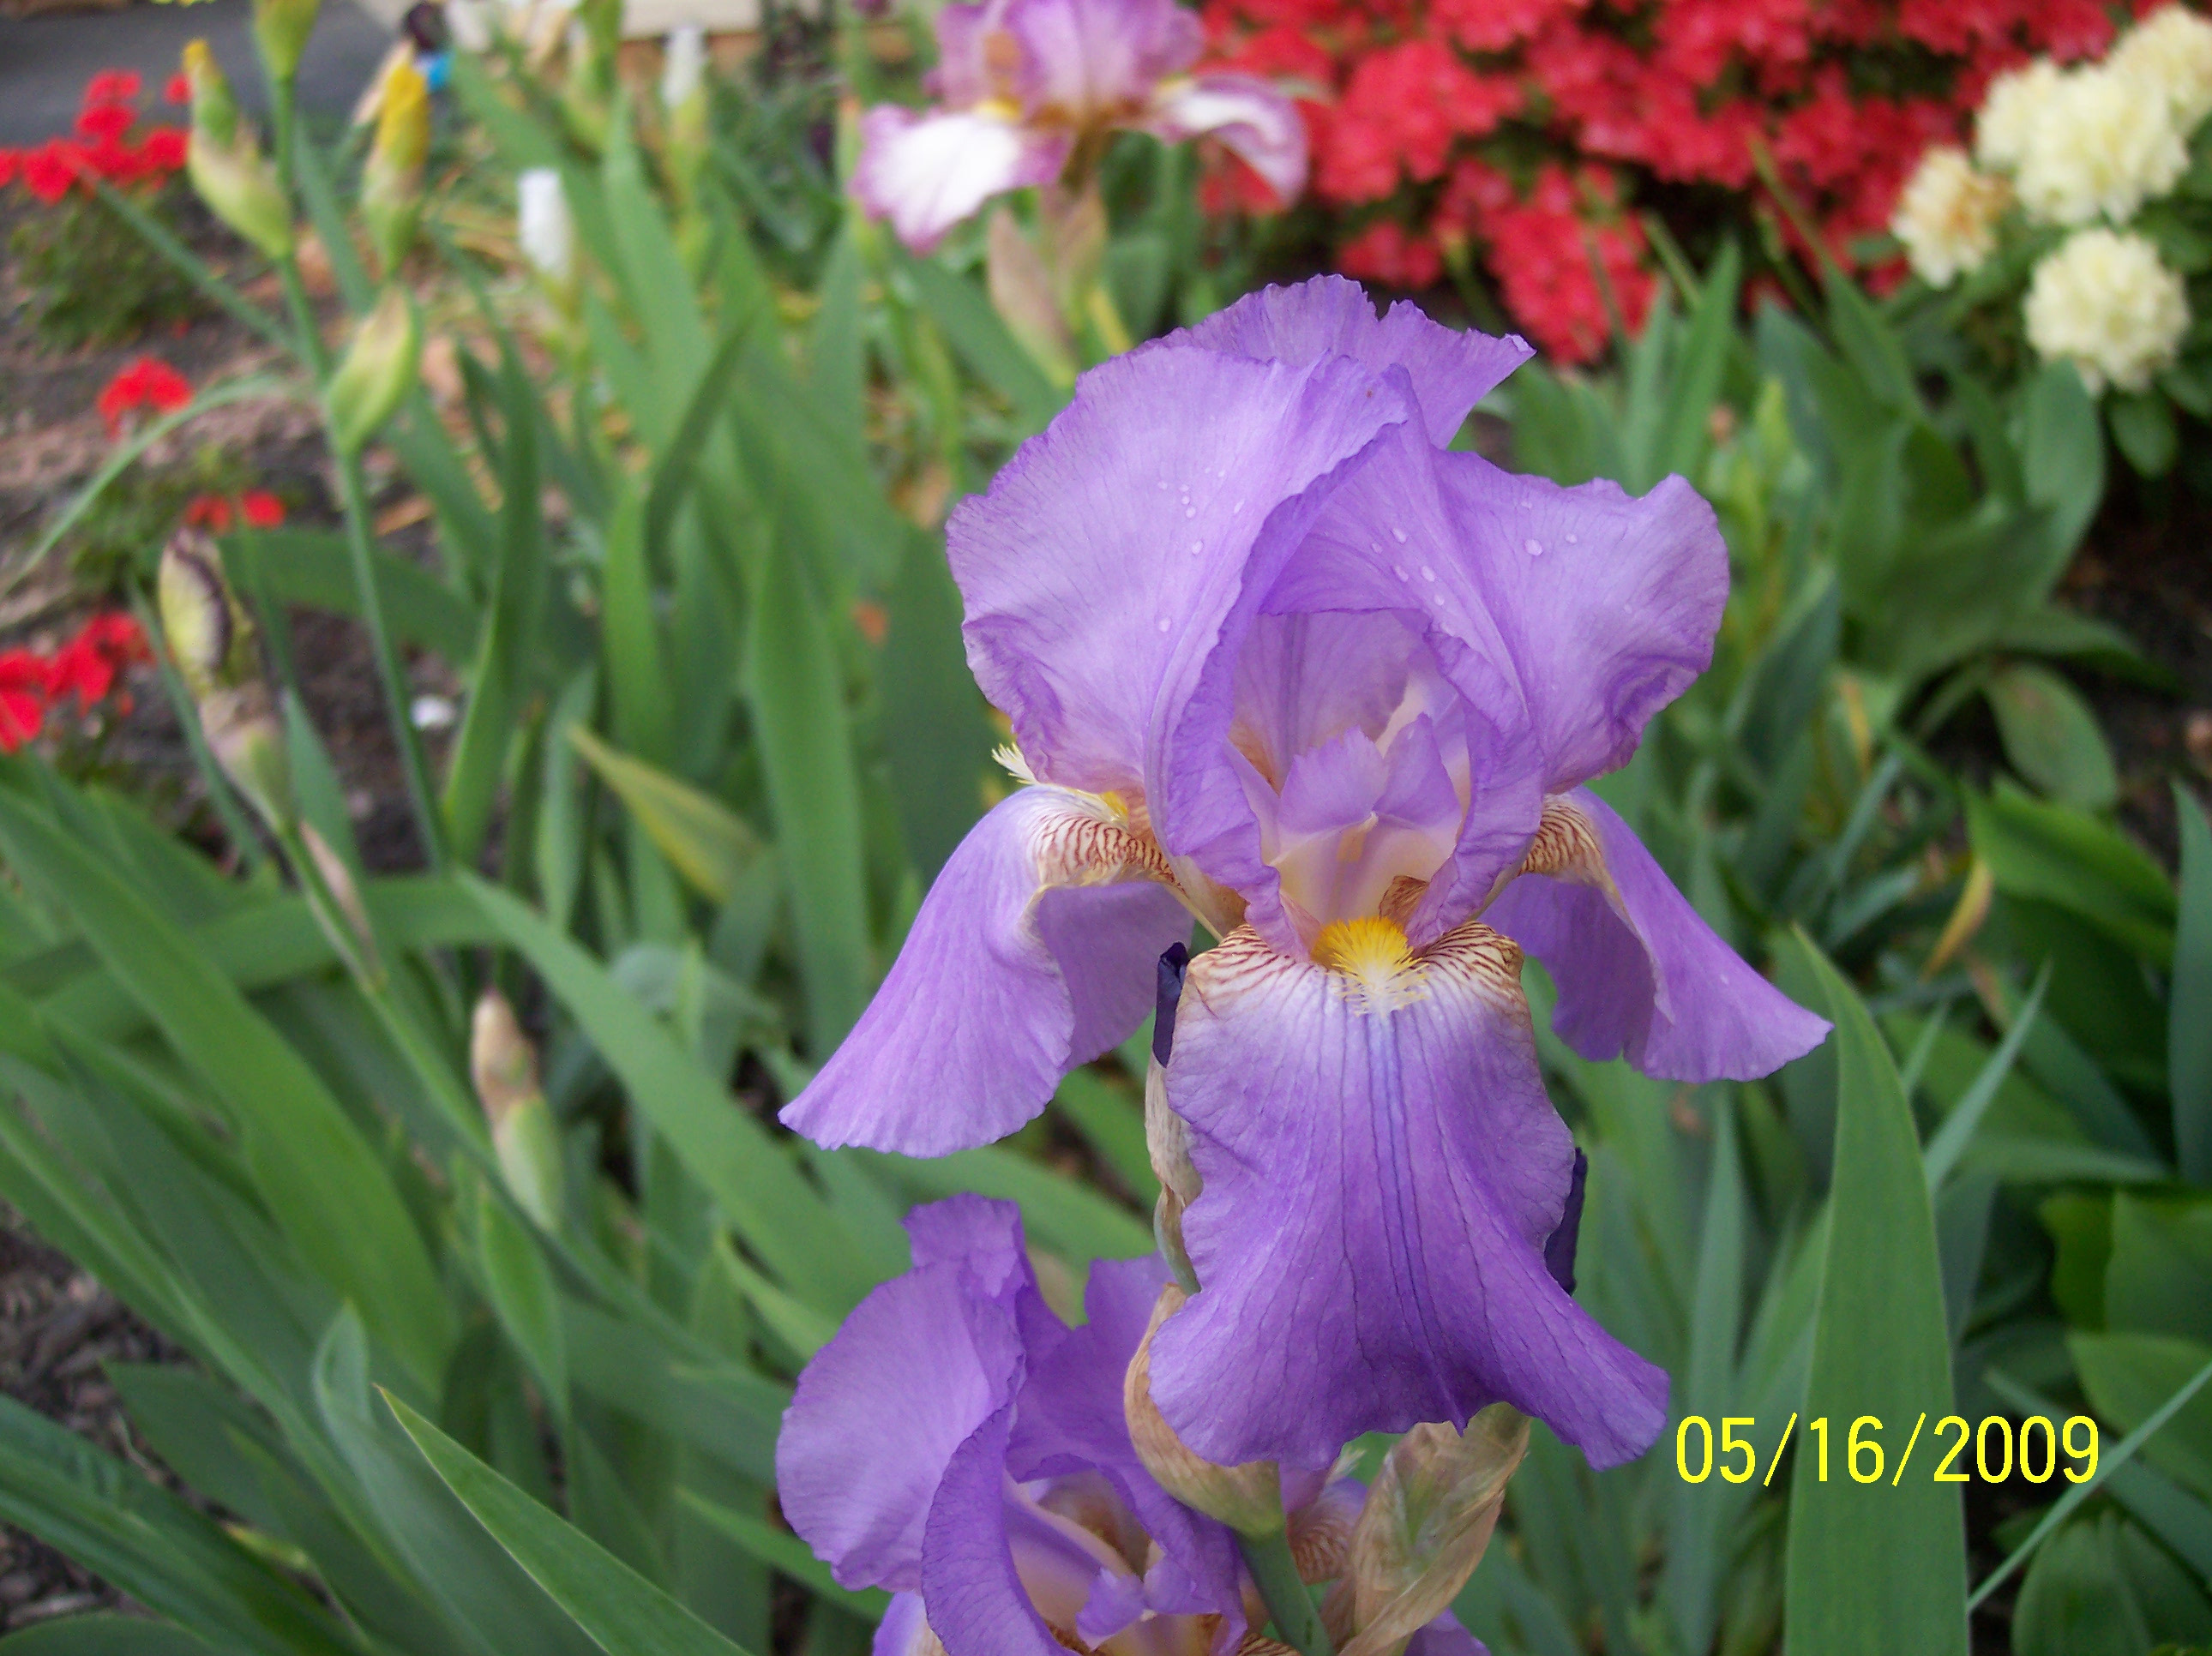
\includegraphics[width=\linewidth]{fig/iris-lavender.jpg}
        \subcaption{Original}
    \end{subfigure}
    \begin{subfigure}{0.45\linewidth}
        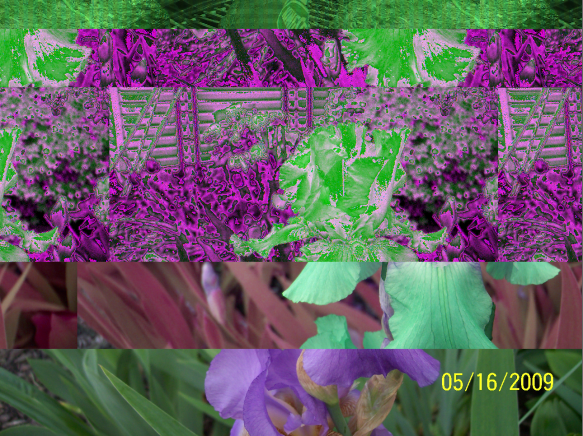
\includegraphics[width=\linewidth]{fig/CR3_fail.png}
        \subcaption{Carved}
    \end{subfigure}
    \caption{
        \emph{iris-lavender.bmp} from the \emph{disorder} test case, as carved by PhotoRec.
        By cross-referencing NIST CFTT's map of the test image with PhotoRec's report file, we find  that the carved file is actually composed of data from 3 files: \emph{iris-lavender.bmp}, \emph{iris-yellow.bmp}, and \emph{smoked-chicken.bmp}.
        In this case, PhotoRec fails to meet FC-CR-03, despite outputting a valid BMP image.
        }
    \label{fig:CR3_fail}
\end{figure}

All tools perfectly fulfil FC-CR-04, meaning every carved file that represents a ``hit,'' is given the same file extension as its corresponding original file.
We limit this only to ``hits,'' excluding false positives, to avoid overlapping with FC-CR-05.

For FC-CR-05, PhotoRec generally scores very high, Foremost and Magnet AXIOM get high scores for some test cases and low scores for others, and Scalpel scores very low for all test cases.
A high score on this core feature means most of the files a tool carves are valid files of some image format and can be properly parsed as that format (we test with the \emph{identify} tool from ImageMagick).
This may imply the tool checks carved files for validity before outputting them.
Note that identify throws a warning for six of the TIFF files used to create CFTT's test images, so we ignore the warning for carved versions of those six files.

\section{Discussion}
In this section, we look at the results from multiple angles. 
We first return to the questions posed in Section~\ref{rqs} to guide our analysis of the chosen DFR tools.
Then, we shift our analysis to the NIST guidelines themselves, by discussing a few situations in which the guidelines are unclear, ambiguous, or misleading.

\subsection{Critique of DFR Tools}
As stated in Section~\ref{rqs}, our objectives are to assess the performance of the DFR tools according to the NIST guidelines, and to determine the factors influencing a tool's success and failure. 

\subsubsection{Performance of Metadata-Based Tools}

None of the tools consistently meet the NIST CFTT guidelines; however, every tool meets the guidelines in some cases.
All tools meet DFR-CR-01 except for TestDisk in one case, where it fails to report a deleted file in metadata.
In that case, the file data is completely overwritten, so the tool may be deliberately choosing to omit the file; however, our interpretation of the guidelines would have it instead return an empty file.
All tools meet DFR-CR-02 without exception, as they attempt to return something for every deleted file.
In some FAT cases, Magnet AXIOM and Autopsy do not recover all data indicated by metadata, so they fail DFR-CR-03.
In many cases, including both file systems and both tools, the recovered file incorrectly contains data from other files, causing the tool to fail DFR-CR-04.
Almost all the times a tool fails to meet the guidelines, it is due to this core feature.


\subsubsection{Conditions for Success of Metadata-Based Tools}

The main factors that cause a metadata-based DFR tool to fail are fragmented files, and overwritten files.
As evidenced by the \emph{basic} case, all tools meet the NIST guidelines when neither of those factors are present.

Most FAT tools detect simple fragmentation in FAT, but Recuva and Magnet AXIOM do not, failing DFR-CR-04 for the \emph{fragments1} case.
When a file is fragmented around another deleted file, all tools fail to detect fragmentation, which means they all fail DFR-CR-04.

Out-of-order fragmentation (the \emph{disorder} cases) in FAT causes all tools to fail to recover the full deleted file, since FAT metadata only provides the location of the first fragment, and it is difficult to detect where the other fragments will be if they are out-of-order.
Three of the tools still meet DFR-CR-03 by just recovering the first fragment, but Autopsy and Magnet AXIOM only return null data or an empty file, failing DFR-CR-03.

Most times a tool fails to meet the guidelines, it specifically fails to meet DFR-CR-04.
This occurs most often in the \emph{overwrite} and \emph{combo} cases, which all feature overwritten deleted files.
In these cases, we expect a tool to not recover anything from the parts of a file that were overwritten, since they now contain a different file's data.
Thus, tools which are more conservative are more likely to meet this core feature (at the risk of failing to meet DFR-CR-04).
The only tool to meet DFR-CR-04 for more than half of the test cases is FTK Imager.
If a deleted file is overwritten by an active file in FAT, FTK Imager returns only up to the point the file was overwritten, then stops.
If a deleted file is overwritten by an active file in NTFS, FTK Imager recovers all the remaining file data, replacing the overwritten part with null data.
In either file system, if all accessible file data is overwritten, FTK Imager returns an empty file.
The only cases where even FTK Imager returns data from the overwriting file are \emph{overwrite4}, \emph{overwrite5}, \emph{overwrite6}, and \emph{combo2}, the cases where the overwriting file has also been deleted.
These cases are difficult for metadata-based DFR tools in general, as the tools tend to rely on file allocation status to detect overwriting (and fragmentation in FAT).

Autopsy fails to meet DFR-CR-03 for the FAT \emph{overwrite2} and \emph{combo1} cases, in which the start of the deleted file is intact but a later part is overwritten.
Instead of recovering all the intact data it can, it simply returns a single cluster.

It may be observed that while DFR-CR-03 and DFR-CR-04 account for almost all the failures, a tool only ever fails to meet one of these core features.
This makes sense as DFR-CR-03 prescribes what a tool should recover at minimum, and DFR-CR-04 prescribes what a tool should not recover.
Thus, meeting the guidelines requires striking a balance between a conservative recovery strategy and a more aggressive one.

\subsubsection{Performance for File Carving Tools}

In most cases, the tools do not fully meet the NIST CFTT expectation; however, they often come close.
All tools meet FC-CR-02 and FC-CR-04 in all cases.

The only case in which a tool fully meets all five core features is PhotoRec on the \emph{nofill} test case.
PhotoRec has by far the best scores for FC-CR-05 and comes close to fully meeting it.
However, it is inconsistent on FC-CR-01 and FC-CR-03.
Foremost gets inconsistent scores on FC-CR-03, but seems to outperform the other tools on this core feature.
Its results on FC-CR-01 mostly mirror PhotoRec's, but are generally lower.
On FC-CR-05, it is inconsistent.

Scalpel consistently recovers at least two thirds of the deleted files, tying with Magnet AXIOM for best average performance on FC-CR-01.
However, it generally performs very poorly on FC-CR-03 and FC-CR-05, though this may be an unfair consequence of our interpretation of the NIST guidelines.
This is discussed in more detail in Section~\ref{sec:false_pos}.

Magnet AXIOM performs about the same as Scalpel on FC-CR-01, consistently carving over two thirds of the deleted files.
Its performance on FC-CR-03 is inconsistent in a similar way to Scalpel's, but with higher scores.
Its performance on FC-CR-05 is inconsistent in a similar way to Foremost, but with mostly higher scores.

Based on our evaluation, no one tool consistently outperforms the others.
Each tool meets some core features very well, and struggles with the rest.
Thus, knowledge and understanding of these trade-offs is important when selecting a file carving tool.




\subsubsection{Conditions for Success of File Carving Tools}

As with metadata-based recovery, the main factors which cause tools to fail are fragmentation and missing data (such as from overwriting).
All tools perform reasonable well on the \emph{basic} and \emph{nofill} cases.
Since these have only complete, contiguous files, they are expected to be easy.
The \emph{simple-frag}, \emph{braid}, and \emph{disorder} cases introduce variations on fragmentation.
Interestingly, almost all tools perform better on braid than on simple-frag.
This makes sense as the files in braid are fragmented around other files, with no space in between, while the files in simple-frag have empty space between the fragments.

A file carving tool can in most cases only detect the start and end of a file, so there is no good way to detect empty space. 
In the braid case, the point of fragmentation is often immediately followed by the start of another file, which the tool can have an easier time detecting.
Since disorder puts the ends of files before their starts, a file carving tool must abandon most reasonable assumptions about the layout of the file system or it will be misled.
Unsurprisingly, this case is very difficult and most tools perform poorly on it relative to the other cases.
The \emph{partials} case introduces missing file data; in this case the missing data is replaced by empty space, rather than overwritten by another file.
This case also seems to be difficult, for the same reasons as simple-frag.

How conservative a tool is about its output has a big impact on its score, particularly for FC-CR-03 and FC-CR-05.
Some tools output a smaller number of files but generally only valid files, while other tools may get more ``hits'' but also output many false positives which do not constitute a valid file.
This is the main reason Scalpel performs so poorly on FC-CR-03 and FC-CR-05 despite its fairly high scores on FC-CR-01.
We believe this represents a flaw in the NIST guidelines, and discuss it in depth in Section~\ref{sec:false_pos}.

One other observation is that Foremost and Magnet AXIOM do not recover any TIFF files from any of the test cases, despite both supporting the format.


\subsection{Critique of NIST Guidelines}
% Metadata
\subsubsection{FAT Fragmentation and Metadata-Based Tools}

To fulfill DFR-CR-03, a tool must recover ``all non-allocated data blocks identified in a residual metadata entry''~\cite{meta:dfr:standards}.
However, in the FAT file system, it's debatable exactly how much is identified in metadata.
Recall that FAT directory entries only store the starting address and the length of a file, and any other information is lost upon file deletion.
So, for a fragmented deleted file, how much should a tool be expected to recover?
Reading DFR-CR-03 very close to the letter, one could argue that the only data definitively identified in metadata is the first cluster; after all, the file could be fragmented between the first and second clusters, and there would be no way to tell from its metadata.
However, this is almost certainly not the intent of the guidelines, as it sets a very low standard for performance.
Since it is possible to reason about the point of fragmentation based on cluster allocation status and other files' metadata, we interpret DFR-CR-03 to mean tools should at least recover the first fragment of a file.
Recovering an entire fragmented file would involve guesswork, so we do not require it.

NIST's James Lyle, who wrote about the challenges of evaluating DFR tools in 2011, 
claims that trying to anticipate the details of every major file system would make the guidelines overly complex. 
Instead, Lyle suggests they be written for `an ideal file system that leaves in 
residual metadata  all  information  required  to  reconstruct  a  deleted  file''~\cite{lyle2011-ICDF2C}, even if this means sometimes holding a tool to an impossible standard.
He further justifies this approach by pointing out that whether a feature is impossible or merely absent, the user experience is the same.
Since the NIST CFTT guidelines seem to have been written with this philosophy in mind, it may not be reasonable to clarify specific edge cases like like the one in this section.
However, the context of this ``ideal file system'' should be explicitly stated in the guidelines document.

\subsubsection{Incompatible Core Features for Metadata-Based Tools}

Under some circumstances, it is impossible for a tool to meet both DFR-CR-03 and DFR-CR-04 at the same time.
For example, suppose a file ``A'' in NTFS is deleted and overwritten, and the file ``B'' that overwrote it is also deleted.
In NTFS, the full run of file A is accessible from metadata after deletion, and since file B was also deleted, all the clusters in file A's run are unallocated.
DFR-CR-03 requires a tool to recover `all non-allocated data blocks identified in a residual metadata entry,''~\cite{meta:dfr:standards} so the entire run of file A should be recovered.
However, this would include data from file B, which is forbidden by DFR-CR-04.
DFR-CR-04 requires that a recovered file contain only data from the ``deleted block pool,'' which is the set of data blocks from the deleted file which ``have not been reallocated or reused.''~\cite{meta:dfr:standards}
Meeting DFR-CR-03 requires recovering data that was reused for file B, so in this case DFR-CR-03 and DFR-CR-04 are incompatible.
This situation occurs in the cases \emph{overwrite4}, \emph{overwrite5}, \emph{overwrite6}, and \emph{combo2} for both FAT and NTFS, and in these cases each tool meets DFR-CR-03 but not DFR-CR-04.
As in the previous section, the user experience is the same regardless of whether or not a task is impossible, so this edge case probably does not justify an update to the guidelines.



% Carving
\subsubsection{False-Positives from File Carving} \label{sec:false_pos}
% What to do about additional files? It's clear for CR1, but not for the others.

All core features for file carving tools besides the first set requirements specifically for all ``carved files.''
The guidelines document defines a carved file as ``a file created by a carving tool purported to be one of the source files present in the search arena.''~\cite{carving_standards}
This means even false positives which are not part of one of the original files affect a tools' evaluation on four out of five of the core features.
We suggest that this results in misleading and less informative results, especially when those results are used to compare different tools.
 
Interpreting ``each carved file'' to include even the ones with no relation to the original files results in dramatically low scores for tools like Scalpel (which carved at least 50 additional ``files'' in most of our tests), while favoring tools which are more conservative in their recovery.
In other terms, this interpretation favors a \emph{strong match policy} over a \emph{weak match policy}.
However, this obscures a relevant trade-off, that a more aggressive tool will have a high false-positive rate, but may recover files that a more conservative tool would miss.
An investigator may have this trade-off in mind when selecting a DFR tool, so the NIST guidelines should not make a tool that sits on one side of that trade-off appear objectively worse than others.

As the standards are currently written, a tool that carves only one file from an image, but recovers it correctly, would be considered perfect on four out of five core features.
Meanwhile, a tool that perfectly carves all 40 files from an image, but also returns 150 false-positives, would likely score very poorly for CF-CR-03, CF-CR-04, and CF-CR-05.
It would score especially poorly on CF-CR-05 as false-positives will almost never be a valid file.
Since the NIST guidelines do not directly account for the false-positive rate, it indirectly and disproportionately affects several core features, diluting their usefulness.

To resolve this issue, we propose the following changes to the NIST guidelines:
\begin{arabiclist}
 \item Add a new definition: \emph{Positive Carved File}, a carved file which corresponds to a supported file header signature from a source file that is present in the search arena.
 \item In CF-CR-03, CF-CR-04, and CF-CR-05, change ``carved file'' to ``positive carved file.''
 \item Add an additional core feature: \emph{The tool shall not return any carved files that do not correspond to a supported file header signature from a source file that is present in the search arena.} This could be scored as the ratio of positive carved files to total carved files.
\end{arabiclist}

The intent of these changes is to better atomize the guidelines, so each core feature evaluates a tool on a single capability.
This should make the trade-offs of certain tools more apparent, enabling investigators to make more informed and nuanced tool choices based on the capabilities that are most important for their use case.

\section{Related Work}

Wu et al.~\cite{wu2020digital} presented a survey on recent advances in the field of DF tools. 
This is a study of the currently available DF tools in general, including file carving tools.

From the experience of designing Scalpel, Richard et al.~\cite{richard2005scalpel} presented 
a set of requirements to fulfill to make a file carving tool perform well. 
Laurenson~\cite{laurenson2013performance} reviewed six file carving tools to evaluate their performance quality.
Interestingly, the research community proposed multiple approaches for file carving. 
For instance, Sencur et al.~\cite{sencar2009identification} exploited bit sequence 
matching to identify fragments of a JPEG file. Furthermore, Gladyshev 
et al.~\cite{gladyshev2017decision} used decision theoretic analysis to carve JPEG files.
Moreover, to recover files from an Ext4 system, Dewald et al.~\cite{dewald2017afeic} built a tool 
that is not solely dependent on metadata information. Their tool uses 
file carving as well as metadata analysis to reconstruct the file.

Lyle~\cite{lyle2011-ICDF2C} proposed a strategy to evaluate metadata-based DFR tools, 
which, in our understanding, NIST CFTT considered while setting the guidelines 
for evaluation of such tools~\cite{meta:dfr:standards}. These guidelines are 
publicly available on the NIST CFTT portal~\cite{cftt:nist}, which we have 
extensively referred to in the current article.

Recently, Lee et al.~\cite{lee2014improved,lee2019extsfr} proposed file recovery techniques based on 
metadata present in an Ext2 or Ext3 file system. Furthermore, the research community has also 
proposed techniques~\cite{nordvik2020generic,atwal2019shining} to carve metadata.

The results and analysis of metadata-based DFR tools in this chapter were originally published in \emph{EAI Endorsed Transactions on Security and Safety} in 2020~\cite{eai}.
Some aspects, such as the naming and organization of test cases, have been reworked to make them more clear and consistent with the file carving cases.
A few redundant test cases from the original have been omitted.
The section on file carving tools is original to this chapter.

\section{Conclusion}\label{conclusion} 

We evaluated deleted file recovery (DFR) tools according to guidelines set by NIST CFTT.
We used test cases provided by CFTT to evaluate file carving tools, and designed our own test cases to evaluate metadata-based DFR tools.
We analyzed the results of these tests to determine how well each tool meets the guidelines and how they compare on various tasks.
We also critiqued the CFTT guidelines based on our experiments and analysis.

In addition to the four core features, there are several optional features listed in the NIST CFTT guidelines for metadata-based DFR tools~\cite{meta:dfr:standards}.
Future work could extend our methodology to evaluate metadata-based tools on these optional features.
Our evaluation of metadata-based tools was limited in scope to just the FAT and NTFS file systems, making it somewhat Windows-centric.
As investigators need to be able to recover evidence from Linux or MacOS devices, future work could evaluate metadata-based tools on ext4, HFS, and other common file systems.
It is common for files to be embedded within other files, for example thumbnails in some graphical formats.
Future work could test the ability of file carving tools to recover these files, and interpret and critique the NIST guidelines in the context of embedded files.
Future work could also extend our investigation of file carving tools beyond just graphical file formats, such as to video or document file formats, which may be equally valuable to an investigation.



%\section*{Acknowledgments}
%Acknowledgments to funding bodies etc. may be placed in a separate
%section at the end of the text, before the Appendices. This should not
%be numbered so use \verb|\section*{Acknowledgements}|.


\bibliographystyle{ws-rv-van}
\bibliography{bibfile}

%\blankpage
%\printindex[aindx]                 % to print author index
%\printindex                        % to print subject index

\end{document} 
